\documentclass[11pt,a4paper]{article}

% ---- Encoding & Fonts ----
\usepackage[utf8]{inputenc}
\usepackage[T1]{fontenc}
\usepackage{lmodern}
\usepackage{microtype}

% ---- Math ----
\usepackage{amsmath, amssymb, amsthm, mathtools}
\usepackage{bm}

% ---- Geometry & Layout ----
\usepackage[margin=1in]{geometry}
\usepackage{setspace}
\usepackage{enumitem}

% ---- Tables & Figures ----
\usepackage{graphicx}
\usepackage{booktabs, multirow, array}
\usepackage{caption}
\usepackage{subcaption}

% ---- TikZ for diagrams ----
\usepackage{tikz}
\usetikzlibrary{positioning, arrows.meta, shapes, fit, calc, decorations.pathreplacing, trees, mindmap, backgrounds}
\usepackage{tikz-cd}

% ---- Algorithms ----
\usepackage{algorithm}
\usepackage{algpseudocode}

% ---- Bibliography ----
\usepackage[numbers, sort&compress, square]{natbib}

% ---- Hyperlinks & References ----
\usepackage[colorlinks=true, linkcolor=blue!60!black, citecolor=teal!70!black, urlcolor=violet]{hyperref}
\usepackage{cleveref}

% ---- Theorem environments ----
\newtheorem{definition}{Definition}[section]
\newtheorem{theorem}{Theorem}[section]
\newtheorem{proposition}{Proposition}[section]
\newtheorem{lemma}{Lemma}[section]
\newtheorem{corollary}{Corollary}[section]
\newtheorem{remark}{Remark}[section]
\newtheorem{example}{Example}[section]
\newtheorem{conjecture}{Conjecture}[section]
\newtheorem{assumption}{Assumption}[section]
\theoremstyle{definition}
\newtheorem{question}{Open Question}[section]
\newtheorem{research}{Research Avenue}[section]
\newtheorem{challenge}{Challenge}[section]

\crefname{question}{Open Question}{Open Questions}
\crefname{research}{Research Avenue}{Research Avenues}

% ---- Custom commands ----
\newcommand{\R}{\mathbb{R}}
\newcommand{\N}{\mathbb{N}}
\newcommand{\Z}{\mathbb{Z}}
\newcommand{\E}{\mathbb{E}}
\newcommand{\Prob}{\mathbb{P}}
\newcommand{\pershom}{\mathrm{PH}}
\newcommand{\PHk}[1]{\mathrm{PH}_{#1}}
\newcommand{\betti}{\beta}
\newcommand{\causaleffect}{\mathrm{CE}}
\newcommand{\Dgm}{\mathrm{Dgm}}
\newcommand{\Dgmk}[1]{\mathrm{Dgm}_{#1}}
\newcommand{\dB}{d_{\mathrm{B}}}
\newcommand{\dW}{W_{\!\infty}}
\newcommand{\Map}{\mathrm{Map}}
\newcommand{\Reeb}{\mathrm{Reeb}}
\newcommand{\Filt}{\mathcal{F}}
\newcommand{\TCDA}{\mathrm{TCDA}}
\newcommand{\SCM}{\mathrm{SCM}}
\newcommand{\Mc}{\mathcal{M}}
\newcommand{\Tc}{\mathcal{T}}
\newcommand{\Cc}{\mathcal{C}}
\newcommand{\Gc}{\mathcal{G}}
\newcommand{\Xc}{\mathcal{X}}
\newcommand{\Yc}{\mathcal{Y}}
\newcommand{\Zc}{\mathcal{Z}}
\newcommand{\doop}{\mathrm{do}}
\newcommand{\ind}{\perp\!\!\!\!\perp}
\newcommand{\given}{\,\vert\,}

\DeclareMathOperator{\ATE}{ATE}
\DeclareMathOperator{\TATE}{TATE}
\DeclareMathOperator{\CATE}{CATE}
\DeclareMathOperator{\GATE}{GATE}
\DeclareMathOperator{\Var}{Var}
\DeclareMathOperator{\Cov}{Cov}
\DeclareMathOperator{\supp}{supp}
\DeclareMathOperator{\Pa}{Pa}

% ---- Title & Authors ----
\title{\textbf{Topological Causal Data Analysis:\\
A Framework for Integrating Persistent Homology\\
with Causal Inference}}
\author{Hugo Gobato Souto\thanks{Dell Technologies. ORCID: \href{https://orcid.org/0000-0002-7039-0572}{0000-0002-7039-0572}. Email: \href{mailto:hugo.souto@dell.com}{hugo.souto@dell.com}} \and Ioannis Diamantis\thanks{Department of Data Analytics and Digitalisation, Maastricht University, Maastricht, The Netherlands. Email: \href{mailto:i.diamantis@maastrichtuniversity.nl}{i.diamantis@maastrichtuniversity.nl}}}
\date{May 2026}

\begin{document}

\maketitle

\begin{abstract}
% Hook
Causal inference enables learning of intervention effects from data, yet modern scientific outcomes are increasingly complex, high-dimensional, and non-Euclidean, undermining the parametric and structural assumptions on which classical causal methods rely. Topological data analysis (TDA) studies the multi-scale shape of data through persistent homology and related functorial constructions, offering descriptors that are provably stable under perturbation but lacking native causal semantics.
% Gap
Despite a growing body of work at their interface---ranging from topologies on the space of structural causal models, to topology-aware treatment-effect estimators, to causal discovery via Hodge decomposition and topological orderings---no unified framework currently organizes these contributions.
% Contribution
This paper proposes \emph{Topological Causal Data Analysis} (TCDA) as a coherent research domain at the intersection of TDA and causal inference. We provide (i) a formal definition of a TCDA problem as a tuple linking a topological space of observations, a causal graph, a topological functor, and a causal query, together with foundational stability and identifiability propositions; (ii) a taxonomy organising existing and prospective work into four domains---topological causal representation, topological robustness in causal inference, causal interpretation of topological features, and methodological applications; (iii) a structured literature review and a suite of five proof-of-concept case studies that instantiate the framework on biomedical imaging, multivariate time series, confounding diagnostics, Mapper-based abstractions, and climate attribution; and (iv) a research agenda comprising eleven formal open questions, fourteen research avenues, and four computational challenges that span theory, computation, applications, and industrial implementation.
% Scope
The paper is designed to be self-contained for researchers from either TDA or causal inference, and aims to catalyse a decade of interdisciplinary work across statistics, machine learning, and the application domains where the shape of data and the structure of cause are intertwined.
\end{abstract}

% Section inputs are activated as each phase is completed.
% See Planning_Phases.md for the build order (Phase 2 onwards).
\IfFileExists{sections/introduction.tex}{\section{Introduction}\label{sec:introduction}

Topological data analysis (TDA) and causal inference (CI) are the two
mathematical languages in which the modern data-analytic enterprise
speaks most precisely about \emph{shape} and about \emph{consequence}.
TDA, developed since the late 1990s, supplies a multi-scale,
functorial, and provably stable grammar for the geometric structure of
data \citep{edelsbrunner2002topological,carlsson2009topology,
edelsbrunner2010computational,wasserman2018topological,
chazal2021introduction}. Causal inference, developed in parallel since
the 1970s, supplies a complete calculus for the interventional and
counterfactual content of probabilistic models
\citep{rubin1974estimating,pearl1995causal,pearl2009causality,
imbens2015causal,peters2017elements,bareinboim2020pearls}. Both fields
have reached methodological maturity; both have generated their own
journals, their own statistical scaffolding, and their own
implementation ecosystems; and both have been applied to many of the
same empirical objects---networks, dynamical systems, biomedical
images, spatiotemporal fields---without explicitly meeting.

The thesis of this paper is that the absence of an explicit meeting
between the two is no longer tenable. Modern scientific data are
increasingly complex, high-dimensional, and non-Euclidean, in ways
that undermine the parametric and structural assumptions on which
classical causal estimators depend; and topological data analysis,
having absorbed a decade of statistical inference results, is now
positioned to deliver not merely descriptive summaries but
\emph{causal} estimators with calibrated uncertainty. A small but
growing body of work---the four seed papers
\citep{ibeling2021topological,kim2026topological,lecci2014statistical,
elyaagoubi2023statistical} that we will treat as the anchors of the
field, together with the sheaf-theoretic causal-inference programme
\citep{mahadevan2021causal,mahadevan2022universal,mahadevan2025sheaf}
and the topological-ordering family of causal-discovery algorithms
\citep{rolland2022score,tran2024constraining,xu2025information,
nocurl2024,wu2026optimization}---has begun to formalise the
connection. What is missing is the framework that organises these
contributions into a single research domain.

We propose such a framework. The remainder of this introduction
positions the contribution: \Cref{sec:intro_parallel} traces the
parallel evolution of TDA and CI; \Cref{sec:intro_why} argues for
their integration; \Cref{sec:intro_limits} states the limitations of
each tradition in isolation; and \Cref{sec:intro_contributions}
enumerates the four contributions that we will make in the body of
the paper.

\subsection{The parallel evolution of two fields}\label{sec:intro_parallel}

Topological data analysis crystallised as a discipline with the
introduction of \emph{persistent homology}: the assignment, to a
filtered simplicial complex, of a multi-set of birth--death pairs that
record the appearance and disappearance of topological features at
each scale \citep{edelsbrunner2002topological,zomorodian2005computing,
edelsbrunner2008persistent}. The stability theorem of
\citet{cohen2007stability}, refined by \citet{chazal2016structure},
established that persistent homology is $1$-Lipschitz with respect to
the bottleneck distance under $L^\infty$ perturbations of the filter,
turning a previously qualitative summary into a calibrated descriptor.
The decade that followed delivered the statistical inference
programme---confidence sets, bootstrap, rates of convergence, and
functional summaries (landscapes, silhouettes, images)---synthesised
in \citet{lecci2014statistical} and consolidated by
\citet{bubenik2015statistical,adams2017persistence,
chazal2014stochastic}. \citet{carlsson2009topology}, the
\citet{singh2007mapper} Mapper algorithm, and the categorical
formalism of \citet{spivak2014category,curry2014sheaves} situated
TDA within a broader functorial-data-analysis programme that
emphasised composability and structure.

Causal inference, in parallel, developed in two complementary
traditions. \citet{rubin1974estimating} and the potential-outcomes
school \citep{rubin2005causal,imbens2015causal} grounded the field in
counterfactual contrasts and identification conditions
(consistency, ignorability, positivity), and produced the
doubly-robust efficient estimation machinery
\citep{robins1989probability,kennedy2024semiparametric,
chernozhukov2018double} that today underwrites empirical work in
biomedicine, econometrics, and policy science. \citet{pearl1995causal,
pearl2009causality,pearl2018book} introduced the structural-causal-
model formalism and do-calculus, which axiomatised intervention as a
syntactic operation on directed acyclic graphs and enabled
\emph{causal discovery}: the recovery of $G$ itself from data via
constraint-based \citep{spirtes2001causation}, score-based
\citep{meek1995strong}, and functional \citep{shimizu2006lingam,
peters2014causal} methods. \citet{bareinboim2020pearls,
ibeling2021topological} crystallised the causal hierarchy
(observational, interventional, counterfactual) into a single
expressive ladder.

\Cref{fig:timeline} in \Cref{sec:literature} traces the two
trajectories side by side. Until $\sim$2020 there is essentially no
crossing: a researcher could attend the major venues of either field
for a decade without hearing the other's vocabulary. The crossings
that began to appear thereafter---a topology on the space of SCMs
\citep{ibeling2021topological}; topology-aware treatment-effect
estimators \citep{kim2026topological}; simulation-based topological
inference for multivariate time series
\citep{elyaagoubi2023statistical}; sheaf-theoretic causal calculi
\citep{mahadevan2021causal,mahadevan2022universal,mahadevan2025sheaf};
and topological-ordering algorithms for causal discovery
\citep{rolland2022score,tran2024constraining,xu2025information,
nocurl2024,wu2026optimization}---are the methodological seeds of the
field this paper proposes to name.

\subsection{Why topology matters for causality}\label{sec:intro_why}

Three properties of topology recommend it as a natural partner for
causal inference, and each is reflected in one of the four domains of
our framework (\Cref{fig:taxonomy}).

\paragraph{Non-Euclidean data.}
The classical average treatment effect, $\ATE = \E[Y^1 - Y^0]$,
implicitly assumes that the difference $Y^1 - Y^0$ is well defined and
scalar-valued. Modern outcomes routinely fail both assumptions: a CT
scan, a molecular conformation, a brain connectivity graph, and a
gridded climate field are all non-Euclidean objects on which
``$Y^1 - Y^0$'' has no obvious meaning. Topological summaries of such
objects---persistence diagrams, Reeb graphs, Mapper complexes---live
in calibrated metric spaces (the Wasserstein space of diagrams, the
interleaving space of Reeb graphs) on which causal contrasts are
well defined \citep{kim2026topological,kurisu2024geodesic}. Sub-domain
A3 of \Cref{sec:framework} (causal embeddings in persistence diagrams)
makes this construction precise.

\paragraph{Robustness through stability.}
The stability theorem (\Cref{eq:stability}) is the operational core of
the field: small perturbations in the data produce only small
perturbations in the persistent invariants, with a constant of one.
This is precisely the kind of bound that classical causal estimators
typically lack and that practical deployment increasingly demands.
\Cref{prop:stability-transfer} shows that any Lipschitz causal
functional of a persistent invariant inherits the quantitative
robustness of $\PHk{k}$, giving a TCDA estimator a tractable
sensitivity guarantee with respect to Hausdorff-scale perturbations
of the data support. Sub-domain B1 of \Cref{sec:framework} formalises
this transfer.

\paragraph{Hidden structure and confounding.}
Unobserved confounders move observed variables along unobserved
orbits and so deposit a topological signature in the joint support
that no graphical or moment-based diagnostic detects. The
worked example of \Cref{sec:cs_confounding}---a hidden circular
confounder generating a persistent $1$-cycle in the residual support
of an apparently null treatment effect---illustrates the principle,
and \Cref{prop:confounding_signature} states it formally. Sub-domain
B2 of \Cref{sec:framework} positions topological diagnostics as a
complement to the meagre-set theorem of
\citet{ibeling2021topological}: where the theorem tells us that
assumption-free identification is impossible on almost all SCMs,
topological diagnostics tell us \emph{which} SCMs have residual
geometric structure consistent with hidden confounding.

These three properties are sufficient to motivate the framework, but
the case for TCDA also rests on a fourth, less elementary observation:
much of modern causal discovery is \emph{already} doing topological
data analysis, often without naming it as such.
\citet{rolland2022score,tran2024constraining,xu2025information,
nocurl2024,wu2026optimization} all extract a topological order from
the data and then refine edges within that order; the order itself is
an invariant of the joint distribution under the appropriate functor,
and \Cref{prop:identifiability} formalises the corresponding
identifiability question. Naming what is already implicit is a small
contribution, but it is one that the field requires before it can
begin to make explicit progress on the deeper questions.

\subsection{Limitations of current approaches}\label{sec:intro_limits}

The case against the status quo is symmetric. Classical causal
inference, applied to non-Euclidean outcomes, must reduce them to
scalar surrogates and so discards exactly the structure of interest;
classical TDA, applied to data with a known causal-graph context,
exposes geometric features but is silent on the question of which
geometric feature carries an intervention's effect. Neither field, on
its own, is equipped to handle a treatment whose outcome is a tumour
shape, a folded protein, a brain network, or a precipitation cluster.

A further limit is structural rather than technical.
\citet{ibeling2021topological}'s topological causal hierarchy theorem
shows that the set of SCMs on which assumption-free identification of
$P(y \mid \doop(x))$ is possible is \emph{topologically meagre}---in
the Baire-category sense, exceptional. This is the topological
counterpart of measure-theoretic ``no-free-lunch'' results
\citep{oxtoby1971measure,belot2020absolutely,genin2017topology,
genin2018topology}, and it places a precise upper limit on what any
purely observational causal procedure can hope to achieve. The
theorem also identifies the structure that must be supplied to do
better, namely a topology on the model space, and is one of the
clearest demonstrations that the language of CI requires topological
extension on its own terms. The complementary critique runs from CI
back to TDA: a persistence diagram is the same whether the variables
it summarises stand in a causal relationship or are mere coincident
features, so without an intervention semantics overlay, a TDA
descriptor cannot license a causal claim. \Cref{sec:lit_gaps}
formalises five specific gaps that follow from this asymmetric
maturity, and \Cref{sec:research} translates each into a concrete
open problem.

\subsection{Our contributions}\label{sec:intro_contributions}

The paper makes four contributions.

\begin{enumerate}[label=(\arabic*),leftmargin=2em]
  \item \textbf{A formal framework.} We propose \emph{Topological
        Causal Data Analysis} (TCDA) as a coherent research domain at
        the intersection of TDA and CI, give a formal definition of a
        TCDA problem as a tuple $(\Mc, G, \Tc, \Cc)$
        (\Cref{def:tcda}), state two foundational propositions
        (\Cref{prop:stability-transfer,prop:identifiability}) that
        establish well-posedness, and defend a taxonomy of four
        top-level domains and twelve sub-domains
        (\Cref{fig:taxonomy}). This is the central intellectual
        contribution and is the subject of \Cref{sec:framework}.

  \item \textbf{A structured literature review.}
        \Cref{sec:literature} synthesises the existing connections
        between TDA and CI along the taxonomy of
        \Cref{sec:framework}, organised across three eras
        (\Cref{sec:lit_early,sec:lit_method,sec:lit_app}) and
        closing with five concrete gaps (\Cref{sec:lit_gaps}). The
        review establishes that every node of the taxonomy is
        already anchored in published work, and that the missing
        piece is the unifying framework we provide.

  \item \textbf{A suite of proof-of-concept case studies.}
        \Cref{sec:case_studies} instantiates the TCDA tuple in five
        concrete settings---biomedical imaging and molecular
        structure (\Cref{sec:cs_tate}), multivariate brain time
        series (\Cref{sec:cs_cycles}), confounding diagnostics
        (\Cref{sec:cs_confounding}), Mapper-based causal abstraction
        with calibrated uncertainty (\Cref{sec:cs_mapper}), and
        spatiotemporal climate attribution
        (\Cref{sec:cs_climate})---together with a worked
        confounding-signature proposition
        (\Cref{prop:confounding_signature}) and a synthesis table
        (\Cref{tab:cs_summary}) mapping each case study back to the
        taxonomy.

  \item \textbf{A research agenda.} \Cref{sec:research} formalises
        eleven Open Questions (\Cref{q:causal-modules}--%
        \Cref{q:topo-docalculus}), fourteen Research Avenues
        (\Cref{r:causal-mapper}--\Cref{r:benchmarks}), and four
        Computational Challenges (\Cref{c:scalable-ph}--%
        \Cref{c:gpu-cubical}), organised into theoretical,
        methodological, computational, domain-specific, and
        industry-facing branches and summarised in the mind-map of
        \Cref{fig:research_mindmap}. Each item is calibrated to be
        specific enough to underwrite an individual research project
        or grant proposal.
\end{enumerate}

\paragraph{What this paper is not.}
TCDA is a proposal, not a theorem. We do not claim that every
component of the framework is mature, that every open question is
solvable, or that the taxonomy is final. Several of the propositions
in \Cref{sec:framework,sec:case_studies} are stated as proof sketches
rather than full theorems, and several of the open questions in
\Cref{sec:research} are likely to be reformulated as the field
matures. The contribution of the paper is to articulate the
framework, locate the existing literature within it, and identify
the questions whose answers will determine whether TCDA becomes a
durable research domain or remains a useful but provisional
re-organisation of work that already exists.

\paragraph{Organisation.}
\Cref{sec:preliminaries} collects the minimal TDA and CI background
needed to read the rest of the paper.
\Cref{sec:framework}~develops the TCDA framework and proves its
foundational propositions. \Cref{sec:literature} surveys the existing
state of the field. \Cref{sec:case_studies} presents five
proof-of-concept case studies. \Cref{sec:research} states the
research agenda. \Cref{sec:conclusion} closes with a call for
interdisciplinary collaboration.
}{}
\IfFileExists{sections/preliminaries.tex}{\section{Preliminaries}
\label{sec:preliminaries}

This section assembles the minimal background needed to read the rest of the
paper. The exposition deliberately addresses two audiences in parallel:
readers fluent in topological data analysis (TDA) who have only passing
familiarity with formal causal inference (CI), and readers fluent in CI who
have only passing familiarity with persistent homology. We therefore strive
for completeness over compression and fix the notation that
\Cref{sec:framework,sec:literature,sec:case_studies,sec:research} will reuse.

\subsection{Topological data analysis}
\label{sec:prelim_tda}

TDA studies the multi-scale geometric and topological structure of data
using tools from algebraic topology
\citep{carlsson2009topology,edelsbrunner2010computational,
chazal2021introduction,wasserman2018topological}. The unifying idea is
\emph{functoriality}: a data set is mapped, in a stable and computable way,
to an algebraic object whose invariants summarise its shape.

\subsubsection{Simplicial complexes and filtrations}

Let $V$ be a finite vertex set. An abstract simplicial complex on $V$ is a
collection $K \subseteq 2^V$ closed under taking subsets: if $\sigma \in K$
and $\tau \subseteq \sigma$, then $\tau \in K$. A simplex
$\sigma \in K$ with $|\sigma| = k+1$ is called a $k$-simplex; the dimension
of $K$ is the maximum dimension of its simplices. A 1-dimensional simplicial
complex is a graph; higher-dimensional simplicial complexes admit triangles,
tetrahedra, and so on.

Given a finite point cloud $X \subset (\Xc, d)$ in a metric space and a
scale parameter $r \ge 0$, the \emph{Vietoris--Rips complex} is
\begin{equation}
  \mathrm{Rips}_r(X)
  = \bigl\{ \sigma \subseteq X : d(u,u') \le 2r \text{ for all } u, u' \in \sigma \bigr\},
  \label{eq:rips}
\end{equation}
and the \emph{\v{C}ech complex} $\mathrm{\check{C}}_r(X)$ collects subsets
whose closed $r$-balls have non-empty common intersection
\citep{hausmann2016vietoris}. For $X \subset \R^m$ the \emph{$\alpha$-complex}
$\mathrm{Alpha}_r(X)$ is built from intersections of Voronoi cells with
$r$-balls and yields a homotopy-equivalent but smaller complex than
$\mathrm{\check{C}}_r$. For image-like grid data, \emph{cubical complexes}
play the analogous role, with elementary cubes replacing simplices.

A \emph{filtration} of $K$ is a nested family
$\Filt = \{K(t)\}_{t \in \R}$ with $K(s) \subseteq K(t)$ whenever
$s \le t$. Increasing $r$ in \cref{eq:rips} produces a Vietoris--Rips
filtration; sublevel sets $K(t) = f^{-1}((-\infty,t])$ of a monotone
function $f : K \to \R$ produce a sublevel filtration. Filtrations
expose the data's structure at multiple resolutions simultaneously.

\subsubsection{Homology and persistent homology}

Singular or simplicial homology assigns to each topological space (or
simplicial complex) $X$ a graded sequence of abelian groups
$H_k(X)$, where $H_0$ counts connected components, $H_1$ counts independent
1-dimensional loops, $H_2$ counts enclosed voids, and so on; the rank of
$H_k(X)$ is the $k$th \emph{Betti number} $\betti_k(X)$
\citep{hatcher2002algebraic,munkres1984elements}. Homology is a functor: a
continuous map $f : X \to Y$ induces a group homomorphism
$H_k(f) : H_k(X) \to H_k(Y)$.

Applied to a filtration $\Filt = \{K(t)\}$, the inclusion
$K(s) \hookrightarrow K(t)$ induces, for every $k$, a linear map
$H_k(K(s)) \to H_k(K(t))$. The collection
$\PHk{k}(\Filt) = \{H_k(K(t))\}_{t \in \R}$ together with these maps is the
\emph{$k$-th persistent homology module} of $\Filt$
\citep{edelsbrunner2002topological,zomorodian2005computing,
edelsbrunner2008persistent}. Over a field, any tame persistent homology
module decomposes uniquely (up to isomorphism) into a direct sum of interval
modules, and the corresponding intervals $[b,d) \subset \R$ form the
\emph{persistence barcode}; equivalently one may record their endpoints as
a multiset of points
\begin{equation}
  \Dgm_k(\Filt) \subset \R^2_+ := \{ (b,d) \in (\R \cup \{\infty\})^2 : b < d \},
  \label{eq:dgm}
\end{equation}
the \emph{persistence diagram} in homology degree $k$
\citep{ghrist2008barcodes,edelsbrunner2010computational}. Following standard
convention, $\Dgm_k$ includes the diagonal $\Delta = \{(t,t) : t \in \R\}$
with infinite multiplicity, so matchings between diagrams may send unmatched
points to $\Delta$.

\subsubsection{Distances on diagrams and the stability theorem}

The two principal metrics on the space of persistence diagrams are the
\emph{bottleneck distance} $\dB$ and the $p$-Wasserstein distance $W_p$:
\begin{equation}
  \dB(D, D') = \inf_{\gamma} \, \sup_{x \in D} \|x - \gamma(x)\|_\infty,
  \qquad
  W_p(D, D') = \Bigl( \inf_{\gamma} \sum_{x \in D} \|x - \gamma(x)\|_\infty^p \Bigr)^{1/p},
  \label{eq:bottleneck}
\end{equation}
where $\gamma$ ranges over bijections $D \cup \Delta \to D' \cup \Delta$.
The cornerstone of statistical TDA is the \emph{stability theorem}: if $f,g$
are tame functions on a triangulable space, then
\begin{equation}
  \dB\bigl(\Dgm_k(f), \Dgm_k(g)\bigr) \le \|f - g\|_\infty,
  \label{eq:stability}
\end{equation}
and analogous bounds hold in Wasserstein distance
\citep{cohen2007stability,chazal2016structure}. Stability is the property
that makes persistent homology a viable summary for noisy data and is what
will allow us, in \Cref{sec:framework}, to lift TDA-level perturbation
guarantees to causal-inference-level robustness statements.

\subsubsection{Functional summaries: landscapes, silhouettes, Euler curves}

For statistical and machine-learning use, it is convenient to embed
$\Dgm_k$ in a Hilbert or Banach space. Three standard embeddings will
appear repeatedly. For $p = (a,b) \in \Dgm_k$, define the tent function
$\Lambda_p(t) = \max\{0, \min(t-a, b-t)\}$. The
\emph{persistence landscape}
$\{\lambda_j(t; D)\}_{j \ge 1}$ records the $j$-th largest value of
$\{\Lambda_p(t)\}_{p \in D}$ \citep{bubenik2015statistical}. The
\emph{power-weighted silhouette} of order $r > 0$ is
\begin{equation}
  \varphi(t; D, r)
  = \frac{\sum_{p = (a,b) \in D} (b - a)^r \, \Lambda_p(t)}
         {\sum_{p = (a,b) \in D} (b - a)^r}, \qquad t \in T \subset \R,
  \label{eq:silhouette}
\end{equation}
with $T$ a fixed compact interval
\citep{chazal2014stochastic,kim2026topological}. The \emph{persistence
image} \citep{adams2017persistence} provides a fixed-dimensional vector
embedding. Finally, the \emph{Euler characteristic curve} records
$\chi(K(t)) = \sum_k (-1)^k \betti_k(K(t))$ along the filtration; though it
discards information, it is cheap to compute and frequently appears in
applications \citep{smith2025multiscale,smith2025harnessing}.

\begin{lemma}[Silhouette Lipschitz stability; informal restatement of
\citealp{kim2026topological}]
\label{lem:silhouette_stability}
Under a uniform bound on tent heights, the power-weighted silhouette
satisfies
$\|\varphi(\cdot; D) - \varphi(\cdot; D')\|_\infty \le c_r \, W_1(D, D')$
for an explicit constant $c_r > 0$ depending only on $r$ and an upper bound
on persistence lifetimes.
\end{lemma}

\Cref{lem:silhouette_stability} is the bridge by which Wasserstein
perturbations of diagrams translate into sup-norm perturbations of
silhouettes; \Cref{sec:framework} uses it to derive causal-stability
statements.

\subsubsection{Mapper and Reeb graphs}

The Mapper algorithm
\citep{singh2007mapper,madukpe2026mapper,dlotko2019ball} produces a
combinatorial summary of a high-dimensional point cloud $X$. Given a
\emph{filter} (or lens) function $f : X \to \R^d$, a cover
$\{U_\alpha\}$ of $f(X)$, and a clustering procedure, Mapper assigns one
node per cluster of $f^{-1}(U_\alpha)$ and connects nodes whose clusters
intersect. The resulting simplicial complex is a discrete proxy for the
Reeb graph of $f$, which collapses connected components of level sets to
points
\citep{biasotti2008reeb,bauer2013measuring,morozov2013interleaving}. Reeb
graphs and Mapper are central in the topological abstraction of causal
mechanisms (\Cref{sec:framework}, Domain A2).

\subsection{Causal inference}
\label{sec:prelim_ci}

Causal inference seeks to quantify what would happen to an outcome under
hypothetical interventions on a system, going beyond the associations
captured by joint distributions
\citep{pearl2009causality,imbens2015causal,peters2017elements,
spirtes2001causation}. Two complementary frameworks dominate the
methodological landscape.

\subsubsection{Structural causal models}

A \emph{structural causal model} (SCM) is a tuple
$\Mc = \langle U, V, \{f_V\}_{V \in V}, P \rangle$, where $V$ is a set of
\emph{endogenous} variables, $U$ a set of \emph{exogenous} variables,
$f_V : \chi_{\Pa(V)} \times \chi_{U(V)} \to \chi_V$ is a measurable
structural function determining each endogenous variable from its parents
and exogenous noise, and $P$ is a Borel probability measure on $\chi_U$
\citep{pearl2009causality,bongers2021foundations,
ibeling2021topological}. Each SCM induces a unique observational
distribution $p^\Mc \in \Prob(\chi_V)$ under recursiveness assumptions;
under an \emph{intervention} $W := w$ on a subset $W \subseteq V$, the
intervened SCM $\Mc_{W := w}$ holds $W = w$ fixed and otherwise leaves
mechanisms intact, yielding an \emph{interventional} distribution
$p^{\Mc_{W := w}}$ \citep{pearl2009causality}.

\emph{Pearl's do-calculus} \citep{pearl1995causal,tian2002general,
lee2019general} provides a complete set of rewrite rules for the
intervention operator $\doop(\cdot)$ on a directed acyclic graph (DAG); it
permits the algorithmic identification of interventional from
observational distributions whenever such identification is possible. The
\emph{causal hierarchy}---observational, interventional, counterfactual---
organises causal queries by the strength of assumption needed to identify
them \citep{bareinboim2020pearls,ibeling2021topological}.

A \emph{causal graph} $G = (V, E)$ on the variable set $V$ encodes the
direct-influence relation: $X \to Y \in E$ means $X \in \Pa(Y)$. We write
$G$ for a generic causal graph and reserve $\Mc$ for SCMs whose graph
structure is $G$. The space of all SCMs compatible with $G$ is denoted
$\mathfrak{M}_G$; without graph restriction we write $\mathfrak{M}$. The
topology on $\mathfrak{M}$ used in \citet{ibeling2021topological} is the
weak topology induced by the convergence of the joint distribution over
all interventions, and is one of the central objects in
\Cref{sec:framework}, Domain B.

\subsubsection{Potential outcomes and causal estimands}

The \emph{potential outcomes} (or Neyman--Rubin) framework
\citep{rubin1974estimating,rubin2005causal,imbens2015causal} parameterises
causal effects directly in terms of counterfactual outcomes. For a binary
treatment $A \in \{0,1\}$ and observed outcome $Y$, one posits
counterfactual outcomes $Y^0, Y^1$ representing the response under each
treatment. The \emph{average treatment effect} is
\begin{equation}
  \ATE = \E[Y^1 - Y^0],
  \label{eq:ate}
\end{equation}
and conditioning on covariates $X$ yields the \emph{conditional average
treatment effect} $\CATE(x) = \E[Y^1 - Y^0 \mid X = x]$. Identification of
\cref{eq:ate} from observational data typically rests on three
assumptions:
\begin{enumerate}[label=(C\arabic*), leftmargin=*]
  \item \emph{Consistency}: $Y = Y^A$ almost surely.
  \item \emph{No unmeasured confounding} (a.k.a.\ ignorability):
        $\{Y^0, Y^1\} \ind A \mid X$.
  \item \emph{Positivity (overlap)}: $0 < \Prob(A = 1 \mid X) < 1$ almost surely.
\end{enumerate}
Under (C1)--(C3), the ATE is identified by
$\ATE = \E[\mu_1(X) - \mu_0(X)]$ with $\mu_a(x) = \E[Y \mid X = x, A = a]$,
and is estimable by inverse-probability weighting, outcome regression, or
\emph{augmented inverse-probability weighting} (AIPW)
\citep{kennedy2024semiparametric,chernozhukov2018double}. AIPW is
\emph{doubly robust}: consistency holds if either the outcome or
propensity model is consistent, and rate-double-robust efficiency holds
under product-rate nuisance conditions
\citep{kennedy2023towards,newey2018cross}.

When the outcome is functional or non-Euclidean, the ATE in \cref{eq:ate}
is no longer well defined, and one must replace the difference of means by
a metric- or geometry-respecting estimand. Two such generalisations recur
in this paper:
\begin{itemize}[leftmargin=*]
  \item the \emph{functional average treatment effect}, defined
        pointwise in a function space and estimated via doubly-robust
        AIPW on the function-on-scalar regression
        \citep{ecker2024causal,testa2025doubly,liebl2023fast};
  \item the \emph{geodesic average treatment effect}, defined in a
        geodesic metric space and estimated via Fréchet means
        \citep{kurisu2024geodesic}.
\end{itemize}
Functional ATEs on \emph{topological} summaries (such as silhouettes) are
exactly what \citet{kim2026topological} formalise, and we will see in
\Cref{sec:framework} that this construction is one of three founding
pillars of the TCDA framework.

\subsubsection{Causal discovery}

Beyond effect estimation, \emph{causal discovery} attempts to learn the
graph $G$ itself from data
\citep{spirtes2001causation,peters2014causal,
shimizu2006lingam,causaldisco2023survey}. Methods fall into three broad
families:
\begin{itemize}[leftmargin=*]
  \item \emph{Constraint-based}: query conditional independencies and
        prune candidate DAGs accordingly (PC, FCI).
  \item \emph{Score-based}: define a regularised likelihood over DAGs and
        search the space (GES, NOTEARS).
  \item \emph{Functional causal models}: exploit functional asymmetries
        such as additive non-Gaussian noise to identify the causal
        direction
        (LiNGAM, ANM).
\end{itemize}
A growing body of work uses \emph{topological orderings} of variables to
shrink the search space
\citep{xu2025information,tran2024constraining,wu2026optimization,
barroso2024inference}; this line is one of the most direct existing
bridges between TDA and CI and is taken up in \Cref{sec:framework},
Domain A1.

\subsection{Existing mathematical bridges}
\label{sec:prelim_bridges}

The interface between TDA and CI is not a void: several mathematical
threads already connect the two communities, although they have not yet
been unified into a single domain. We review three.

\subsubsection{Topologies on causal-model spaces}

Following \citet{dembo1994topological} and \citet{genin2017topology},
open sets of the weak topology on probability distributions correspond to
statistically \emph{verifiable} hypotheses. \citet{ibeling2021topological}
extend this correspondence to the space of SCMs by constructing a sequence
of topologies, one for each level of the causal hierarchy, and proving
that the collapse set of the hierarchy is topologically meager. Earlier
parametric results on faithfulness violations
\citep{meek1995strong,uhler2013geometry} can be re-read in this light as
measure-theoretic predecessors to the topological statement. We use the
phrase ``topology of causal models'' for this line of work and adopt it
as the foundation of \Cref{sec:framework}, Domain B.

\subsubsection{Sheaf-theoretic and categorical approaches}

Sheaves, originally developed for cohomology and complex geometry
\citep{bredon1997sheaf}, have re-emerged as a language for distributed
data, signal processing, and now causal inference
\citep{robinson2014topological,curry2014sheaves,spivak2014category}.
\citet{mahadevan2021causal,mahadevan2022universal,mahadevan2025sheaf}
develop a topos-theoretic formulation of causal inference in which
do-calculus is generalised via subobject classifiers, the space of causal
DAGs is endowed with an Alexandroff topology, and certain identification
results take the form of sheaf-cohomology statements. Independently, the
categorical view of persistent homology---homology is a functor, and
filtrations are functors from $(\R, \le)$ to the category of topological
spaces---suggests that any \emph{functorial} causal inference procedure
should commute, up to a controllable error, with the topological functor
used to summarise data. This is the formal content of Domain B3
(``functorial causal inference'') in \Cref{sec:framework}.

\subsubsection{Optimal transport and Wasserstein space}

Optimal transport equips spaces of probability measures with rich
geometric structure
\citep{villani2009optimal,peyre2019computational}. Two threads concern
this paper. First, persistence diagrams are themselves compared via
$W_p$-distances; many statistical guarantees for persistent homology are
expressed in these terms
\citep{mileyko2011probability,turner2014frechet,
chazal2014stochastic}. Second, the Wasserstein distance offers a natural
metric on counterfactual distributions and so on causal effect
estimators, with stability results connecting changes in observed
distributions to changes in identified causal quantities. The combination
of these two threads underwrites the silhouette stability bound of
\citet{kim2026topological}, which we will use in
\Cref{sec:framework}.

\subsection{Notation summary}
\label{sec:notation}

We collect the notation that recurs throughout the paper.

\begin{center}
\begin{tabular}{@{}lp{0.78\linewidth}@{}}
\toprule
Symbol & Meaning \\
\midrule
$(\Mc, d)$       & Topological / metric space of observations (a Polish space, in the broadest setting). \\
$\Filt = \{K(t)\}_{t \in \R}$ & A filtration of simplicial / cubical complexes built from data. \\
$\PHk{k}(\Filt)$ & $k$-th persistent homology module of the filtration. \\
$\Dgm_k(\Filt)$  & $k$-th persistence diagram (multiset of birth--death pairs). \\
$\dB, \dW, W_p$  & Bottleneck and $p$-Wasserstein distances on diagrams. \\
$\varphi(t; D, r)$ & Power-weighted silhouette function of diagram $D$ at exponent $r$. \\
$\Map_f, \Reeb_f$ & Mapper and Reeb-graph summaries with filter $f$. \\
$G = (V, E)$     & Causal graph (directed acyclic, unless stated). \\
$\Mc \in \mathfrak{M}_G$ & SCM with graph $G$; $\mathfrak{M}$ if the graph is unspecified. \\
$p^\Mc, p^{\Mc_{W := w}}$ & Observational and interventional distributions of $\Mc$. \\
$Y^a$             & Potential outcome under treatment $A = a$. \\
$\ATE, \CATE, \TATE, \GATE$ & Average / conditional / topological / geodesic ATEs. \\
$\Tc$            & A topological functor (persistent homology, Mapper, etc.) acting on data. \\
$\Cc$            & A causal query (e.g., $\ATE$, $\doop$-expression, identifiability question). \\
$\TCDA$          & Topological Causal Data Analysis (the proposed domain). \\
\bottomrule
\end{tabular}
\end{center}

This notation is used uniformly in \Cref{sec:framework} onwards. The
quadruple $(\Mc, G, \Tc, \Cc)$ in particular will be the carrier of the
TCDA formalism.

\medskip

Equipped with these tools, we now turn to the main intellectual
contribution of the paper.
}{}
\IfFileExists{sections/framework.tex}{\section{The TCDA Framework}\label{sec:framework}

Building on the preliminaries of \Cref{sec:preliminaries}, we now propose
\emph{Topological Causal Data Analysis} (TCDA) as a coherent research
domain at the intersection of TDA and causal inference. Our exposition
proceeds in five steps. \Cref{sec:formal-tcda} gives a formal definition
of a TCDA problem as a tuple linking a topological space of observations
to a causal graph through a functorial topological summary, together with
two foundational propositions establishing well-posedness.
\Cref{sec:domain-A,sec:domain-B,sec:domain-C,sec:domain-D} then defend a
four-domain taxonomy: representation (A), robustness (B), interpretation
(C), and methodology (D), each with three sub-domains. The taxonomy is
summarised in \Cref{fig:taxonomy} and is the paper's primary intellectual
contribution. Every sub-domain is anchored to at least one published
work, ensuring that the framework is grounded rather than aspirational.

\subsection{Formal definition of a TCDA problem}\label{sec:formal-tcda}

The unifying intuition is that, in a TCDA problem, causal inference is
performed not on raw observations but on \emph{topological summaries} of
those observations, where the summary is computed by a functor that
satisfies the stability and interpretability properties recalled in
\Cref{sec:prelim_tda}. The causal question of interest is then either
(i)~a query about the underlying causal structure that generated the
observations, or (ii)~a contrast between topological summaries induced
by different interventions, or (iii)~a robustness/identifiability
statement about classical causal estimands whose validity is controlled
by topological invariants.

\begin{definition}[TCDA problem]\label{def:tcda}
A \emph{topological causal data analysis problem} is a tuple
\[
\TCDA \;=\; (\Mc,\, G,\, \Tc,\, \Cc),
\]
whose components are:
\begin{enumerate}[leftmargin=2em,label=(\roman*)]
\item $\Mc$ is a (Polish) topological space of observations equipped with
a metric or filtration parameter $\rho:\Mc\times\Mc\to\R_{\geq 0}$, on which
probability measures and their interventional counterparts are well-defined;
\item $G = (V,E)$ is a causal structure---typically a DAG or ADMG---whose
vertices represent (possibly latent) random variables $X = (X_v)_{v\in V}$
taking values in $\Mc$ and whose edges encode direct causal relationships
in the SCM sense of \Cref{sec:prelim_ci};
\item $\Tc \,:\, \mathbf{Filt}(\Mc) \,\to\, \mathbf{Pers}$ is a
\emph{topological functor} from a category of filtered objects on $\Mc$
to a category of persistence-like invariants. Canonical instances are
$\Tc = \PHk{k}$ for $k\in\{0,1,2\}$, $\Tc = \Reeb_f$, $\Tc = \Map_f$,
and their functional summaries $\Tc = \varphi(\cdot;\,r)$ (silhouettes)
or $\Tc = \Lambda$ (landscapes). We require $\Tc$ to be stable with
respect to some interleaving-type metric on $\mathbf{Filt}(\Mc)$;
\item $\Cc$ is a \emph{causal query}---a functional of the
interventional or counterfactual distribution induced by $G$ on $\Mc$.
We allow $\Cc$ to act directly on raw outcomes ($\Cc = \ATE,\CATE,\TATE,
P(y\mid \doop(x)),\ldots$) or on topological summaries
($\Cc = W_p(\Dgmk{k}(P^{x}),\Dgmk{k}(P^{x'}))$, for example, as in
\citet{kim2026topological}).
\end{enumerate}
A TCDA \emph{solution} is an estimator $\widehat\Cc_n$ together with
calibrated uncertainty (confidence sets, hypothesis tests, posterior
credible sets) for the population quantity $\Cc$, computed from a sample
$\{X_i\}_{i=1}^n \subset \Mc$ using $\Tc$ as a (possibly sufficient)
statistic.
\end{definition}

\Cref{def:tcda} is intentionally broad. The four components
$(\Mc, G, \Tc, \Cc)$ play orthogonal roles: $\Mc$ specifies \emph{what
the data is}, $G$ specifies \emph{which causal relationships are
admitted}, $\Tc$ specifies \emph{how shape is summarised}, and $\Cc$
specifies \emph{the scientific question}. Existing work occupies
distinct corners of this space:
\begin{itemize}[leftmargin=2em]
\item \citet{ibeling2021topological} take $\Tc$ to be the identity and
endow $\Mc = \mathfrak{M}$ (a space of SCMs) with a topology that controls
the Pearl--Bareinboim causal hierarchy.
\item \citet{kim2026topological} fix $\Cc$ to be a Wasserstein contrast
between persistence diagrams of potential outcomes and develop AIPW
estimators with $\sqrt n$-rates and weak-convergence guarantees.
\item \citet{elyaagoubi2023statistical} fix $\Mc$ to be a space of
multivariate time-series, $\Tc = \PHk{1}$ of a windowed dependence
network, and $\Cc$ to be a hypothesis test about the number of cycles.
\item \citet{lecci2014statistical} develops the calibrated statistical
inference for $\Tc$ alone that any TCDA estimator must inherit.
\end{itemize}
Thus the four seed works of the field each fix three components of the
TCDA tuple and study the remaining one. The TCDA programme is precisely
the systematic study of the joint behaviour of all four.

% =====================================================================
% Figure: TCDA Taxonomy (Section 3.1)
% This is a working draft. The user has indicated that final figure
% production will be handled separately; the file is provided so the
% document compiles and the cross-reference \Cref{fig:taxonomy} resolves.
% =====================================================================
\begin{figure}[t]
\centering
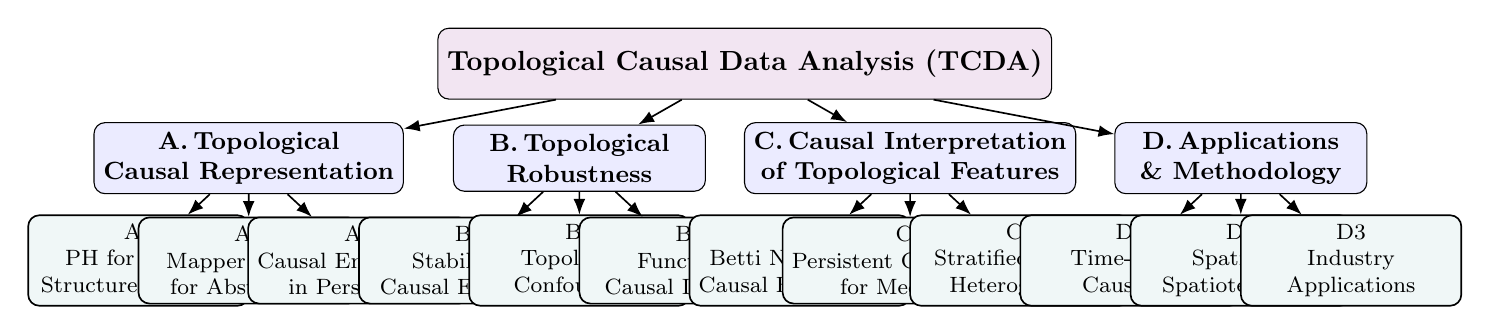
\begin{tikzpicture}[
  font=\small,
  level distance=11mm,
  level 1/.style={sibling distance=42mm, level distance=12mm,
                  every node/.style={draw, rounded corners, fill=blue!8,
                                     align=center, minimum width=32mm,
                                     minimum height=7mm, font=\small\bfseries}},
  level 2/.style={sibling distance=14mm, level distance=13mm,
                  every node/.style={draw, rounded corners, fill=teal!6,
                                     align=center, minimum width=28mm,
                                     minimum height=6mm, font=\footnotesize}},
  edge from parent/.style={draw, -{Latex[length=2mm]}, semithick}]

\node[draw, rounded corners, fill=violet!10, minimum width=64mm,
      minimum height=9mm, font=\bfseries] {Topological Causal Data Analysis (TCDA)}
  child {node {A.\,Topological\\Causal Representation}
    child {node {A1\\PH for Causal\\Structure Learning}}
    child {node {A2\\Mapper \& Reeb\\for Abstraction}}
    child {node {A3\\Causal Embeddings\\in Persistence}}
  }
  child {node {B.\,Topological\\Robustness}
    child {node {B1\\Stability of\\Causal Estimates}}
    child {node {B2\\Topological\\Confounding}}
    child {node {B3\\Functorial\\Causal Inference}}
  }
  child {node {C.\,Causal Interpretation\\of Topological Features}
    child {node {C1\\Betti Numbers as\\Causal Explanation}}
    child {node {C2\\Persistent Cohomology\\for Mediation}}
    child {node {C3\\Stratified Causal\\Heterogeneity}}
  }
  child {node {D.\,Applications\\\& Methodology}
    child {node {D1\\Time-Series\\Causality}}
    child {node {D2\\Spatial \&\\Spatiotemporal}}
    child {node {D3\\Industry\\Applications}}
  };
\end{tikzpicture}
\caption{The proposed TCDA taxonomy. Four orthogonal domains, each with
three sub-domains, organise the field. Domain A concerns
\emph{representation}: how topology summarises the structure of causal
data. Domain B concerns \emph{robustness}: how topological stability
controls the sensitivity of causal estimates to perturbations. Domain C
concerns \emph{interpretation}: which causal stories are encoded by
topological features. Domain D concerns \emph{methodology and applications}
in concrete data modalities. The taxonomy is intended to be exhaustive
(every existing TCDA contribution we are aware of fits in at least one
node) but not mutually exclusive (many works contribute to several
sub-domains simultaneously).}
\label{fig:taxonomy}
\end{figure}


\paragraph{Requirements on $\Tc$.}
For \Cref{def:tcda} to be useful in a causal context, the functor $\Tc$
must satisfy three operating conditions:
\begin{enumerate}[leftmargin=2em,label=(F\arabic*)]
\item \emph{Stability.} Small perturbations of the input filtration
should produce small perturbations of $\Tc(\cdot)$ in an interleaving-type
metric. Persistent homology satisfies this with constant $1$ for the
bottleneck distance (\Cref{eq:stability}). Mapper and Reeb functors
admit weaker but useful stability properties under appropriate
discretisation \citep{munch2016convergence,carriere2018statistical}.
\item \emph{Interpretability.} The features of $\Tc(\cdot)$ should admit
a substantive interpretation in the underlying scientific domain (e.g.,
$1$-cycles in $\PHk{1}$ of a brain functional network correspond to
re-entrant cortical loops; \citealp{elyaagoubi2023statistical,
sizemore2018cliques}).
\item \emph{Computability.} The functor must be computable in time
polynomial in the sample size for the kind of data the application
demands. Off-the-shelf libraries \texttt{Ripser}, \texttt{GUDHI},
\texttt{giotto-tda} provide $O(n^3)$ persistent-homology computation up
to dimension $2$ in practice; sparse and approximate variants extend
this to $n \gtrsim 10^5$ \citep{bauer2021ripser,otter2017roadmap,
tauzin2021giotto}.
\end{enumerate}
We refer to functors satisfying (F1)--(F3) as \emph{admissible} and
restrict attention to admissible $\Tc$ in all that follows.

We now state two propositions that establish the well-posedness of the
TCDA tuple. The first transfers the celebrated stability of persistent
homology to any Lipschitz causal query; the second pins down the
informational condition under which a causal graph is identifiable from
a topological functor alone. Both are stated for the canonical case
$\Tc = \PHk{k}$ but extend immediately to silhouettes, landscapes, and
other Lipschitz functional summaries.

\begin{proposition}[Stability transfer]\label{prop:stability-transfer}
Let $\TCDA = (\Mc, G, \Tc, \Cc)$ be a TCDA problem with $\Tc = \PHk{k}$
applied to the Vietoris--Rips filtration of a compact subset of $\Mc$,
and let
\[
  \Cc\bigl[\Tc(P), \Tc(Q)\bigr] \;=\; \phi\bigl(\Dgmk{k}(P),\,\Dgmk{k}(Q)\bigr)
\]
for some functional $\phi$ that is $L$-Lipschitz with respect to the
$p$-Wasserstein distance on persistence diagrams. Then for any pair of
distributions $P, P' \in \mathcal{P}(\Mc)$ with bounded support and any
fixed $Q$,
\[
\bigl|\Cc[\Tc(P),\Tc(Q)] - \Cc[\Tc(P'),\Tc(Q)]\bigr|
\;\leq\; L \cdot W_p\!\bigl(\Dgmk{k}(P),\,\Dgmk{k}(P')\bigr)
\;\leq\; L \cdot d_H\!\bigl(\supp P,\, \supp P'\bigr),
\]
where $d_H$ denotes the Hausdorff distance between the supports of $P$
and $P'$.
\end{proposition}

\begin{proof}[Sketch]
The first inequality is the Lipschitz assumption on $\phi$; the second
is the stability theorem for persistent homology
(\Cref{eq:stability}; \citealp{cohen2007stability,chazal2016structure}).
The constant is $1$ in the canonical bottleneck case and tracks the
$p$-Wasserstein constant otherwise.
\end{proof}

\emph{Significance.} \Cref{prop:stability-transfer} says that any causal
query expressible as a Lipschitz functional of persistence diagrams
inherits the quantitative robustness of $\PHk{k}$: a small Hausdorff
perturbation of the support---a much weaker requirement than convergence
in any parametric metric---bounds the perturbation of the causal
estimand. This delivers a robustness guarantee with no analogue in
classical (parametric) causal inference. \citet{kim2026topological}
exploit precisely this transfer to establish stability of their TATE
estimator under the silhouette-based summary $\Tc = \varphi(\cdot;r)$.

\begin{proposition}[Identifiability from a topological functor]
\label{prop:identifiability}
Let $G$ vary over a class $\mathcal{G}$ of DAGs over the random vector
$X$, let $\mathcal{P}_G$ denote the observational distribution induced by
$G$, and let $\Tc$ be an admissible topological functor. Then $G$ is
identifiable from $\Tc(\mathcal{P}_G)$ alone---i.e., there is a function
$\Psi$ such that $\Psi(\Tc(\mathcal{P}_G)) = G$ for all $G \in \mathcal{G}$
\emph{if and only if} the assignment $G \mapsto \Tc(\mathcal{P}_G)$ is
injective on $\mathcal{G}$.
\end{proposition}

\begin{proof}[Sketch]
The ``only if'' direction is immediate: if the map is non-injective,
then two distinct $G_1 \neq G_2$ produce identical $\Tc(\cdot)$, so no
inverse $\Psi$ exists. The ``if'' direction is the definition of
identifiability: an injective map admits a left inverse on its image,
and any such left inverse plays the role of $\Psi$. Standard measurable
selection (e.g., the Kuratowski--Ryll-Nardzewski theorem) supplies a
measurable $\Psi$ when $\mathcal{G}$ is countable, as in the
finite-DAG case.
\end{proof}

\emph{Significance.} \Cref{prop:identifiability} isolates the exact
informational condition under which a topology-based discovery algorithm
can hope to recover the underlying graph. It allows existing
topology-based discovery procedures to be classified by what $\Tc$ they
implicitly use: TOPIC \citep{tran2024constraining} uses the
score-Jacobian functor, SSTS \citep{xu2025information} uses a mutual-
information-based functor, and Hodge-decomposition methods
\citep{nocurl2024} use the harmonic component of a $1$-chain. The
proposition does not, of course, certify that the injectivity condition
\emph{holds} for a given $\Tc$; we list this as
\Cref{q:tcda-identifiability} in \Cref{sec:research}.

\medskip
Together, \Cref{prop:stability-transfer,prop:identifiability} establish
that the TCDA tuple is non-vacuous: it inherits both the stability and
the identifiability properties that motivate its definition. The
remaining sections of this section show that the four domains of the
taxonomy fall out naturally as the four ``faces'' of \Cref{def:tcda}---one
for each of the components $\Tc$, $\Cc$ in their representational and
robustness roles, plus one for the interpretive direction (reading
causality \emph{out} of $\Tc$) and one for the methodological direction
(applying TCDA in specific data modalities).

\subsection{Domain A: Topological Causal Representation}\label{sec:domain-A}

Domain A addresses the question: \emph{which topological structure best
represents the causal content of high-dimensional, non-Euclidean data?}
The role of $\Tc$ in \Cref{def:tcda} is here that of a sufficient
statistic for the causal structure or for the interventional contrasts
of interest. Three sub-domains arise.

\subsubsection*{A1. Persistent homology for causal structure learning.}
Persistent homology of a multivariate distribution or its empirical
dependence graph can serve as a sufficient statistic for the underlying
causal DAG. Two threads converge here. First, modern \emph{topological-
ordering} approaches to causal discovery---e.g.\ TOPIC
\citep{tran2024constraining}, SSTS \citep{xu2025information}, NoCurl-X
\citep{nocurl2024}, OptiTopo \citep{wu2026optimization}, and CaPS
\citep{rolland2022score}---use rank-based or information-theoretic
functors to extract a topological order from the data and then refine
edges within that order; the order itself is a topological invariant of
the joint distribution. Second, persistent homology of the
\emph{dependence network} of a multivariate time series identifies
feedback cycles \citep{elyaagoubi2023statistical}; loops in
$\PHk{1}$ correspond to directed feedback loops in the underlying
Granger graph, and a generative simulation framework
\citep{elyaagoubi2023statistical} now exists to test how well
TDA-based discovery methods recover known cycle structure. In the
language of \Cref{prop:identifiability}, sub-domain A1 chooses $\Tc$ to
satisfy the injectivity condition for restricted classes of $G$ (e.g.\
additive-noise models with non-Gaussian innovations).

\subsubsection*{A2. Mapper and Reeb graphs for causal abstraction.}
Where A1 produces a graph that approximates $G$, A2 produces a
\emph{topological abstraction} of the underlying causal mechanism: a
simplification of the data space along a filter function chosen to
align with the causal structure. The Mapper algorithm
\citep{singh2007mapper,carriere2018statistical} partitions $\Mc$ along
level sets of a filter $f$ and glues the resulting clusters into a
simplicial complex; under appropriate choices of $f$, the resulting
complex captures coarse causal regimes (treatment-response strata,
phase transitions, mechanism-shift points). Reeb graphs play the
analogous role for continuous filters \citep{biasotti2008reeb,
morozov2013interleaving}. The recent ball-mapper variant
\citep{dlotko2019ball} is particularly attractive for causal abstraction
because it bypasses the cover-selection problem and admits a stability
guarantee. The statistical scaffolding of \citet{lecci2014statistical}
applies directly: bootstrap confidence sets on cluster trees yield
calibrated abstractions, which is essential when the abstraction is to
serve as the carrier of a downstream causal query.

\subsubsection*{A3. Causal embeddings in persistence diagrams.}
Sub-domain A3 represents the \emph{causal effect itself} as a
topological feature: each potential outcome distribution $P^a$ is
summarised by a persistence diagram $\Dgmk{k}(P^a)$ (or its silhouette
$\varphi(\cdot;P^a,r)$) and the causal contrast is a distance,
hypothesis test, or learned mapping between these diagrams. This is
exactly the formulation of \citet{kim2026topological}, who define the
\emph{topological average treatment effect}
\[
\TATE = W_1\!\bigl(\Dgmk{k}(P^{a=1}),\,\Dgmk{k}(P^{a=0})\bigr),
\]
and provide an AIPW estimator with $\sqrt n$-rate. The same idea applies
in non-Euclidean outcome spaces: the geodesic ATE of
\citet{kurisu2024geodesic} for Riemannian-valued outcomes admits a
topological generalisation in which the Fr\'echet mean is replaced by
the persistence diagram. Sub-domain A3 thus exhibits the TCDA tuple in
its most direct form: $\Tc$ converts outcomes to diagrams; $\Cc$ is a
metric or test on those diagrams; the causal graph $G$ underwrites
identifiability of the contrast.

\subsection{Domain B: Topological Robustness in Causal Inference}\label{sec:domain-B}

Domain B addresses the question: \emph{when can topological invariants
\textbf{control} the sensitivity of causal estimates to perturbations of
the data, the model, or the identifying assumptions?} Here the role of
$\Tc$ is to deliver Lipschitz-type bounds that propagate to $\Cc$.

\subsubsection*{B1. Stability of causal estimates under topological perturbations.}
\Cref{prop:stability-transfer} is the prototype: any Lipschitz causal
query whose primary statistic is a persistence diagram inherits a
quantitative robustness bound from the bottleneck/Wasserstein stability
of $\PHk{k}$. \citet{kim2026topological} exploit this in their stability
theorem for the silhouette TATE; \citet{farzam2025topology} extend it to
representation-learning settings where topological summaries serve as
distributionally-robust losses. A complementary thread uses persistence
landscapes \citep{bubenik2015statistical} as smooth, Hilbert-space-valued
embeddings, which allows classical M-estimation rates to be transferred
to TDA-based causal estimators. The statistical inference programme of
\citet{lecci2014statistical}---confidence sets, bootstrap, rates of
convergence on landscapes and diagrams---is the inferential backbone of
all B1 work: a TCDA estimator that lacks calibrated uncertainty cannot
deliver causal robustness, only descriptive plots.

\subsubsection*{B2. Topological detection of unobserved confounding.}
A persistent ``hole'' in the data manifold can betray the action of an
unobserved variable: when an unobserved confounder $U$ moves an outcome
along an orbit, the support of the observed distribution exhibits a
non-trivial $\PHk{1}$ class that the observed graph cannot explain. This
observation has been operationalised in two ways. First, \emph{anomaly
scores} based on bottleneck or Wasserstein distance flag samples whose
local persistence diagram differs from the population diagram
\citep{bruel2018topological,nigmetov2022topological}; flagged samples
are candidates for hidden-confounder action. Second, the topological
hierarchy of \citet{ibeling2021topological} shows that the set of SCMs
for which an assumption-free identification of $P(y\mid \doop(x))$ is
possible is \emph{topologically meager}, formalising the intuition that
confounders are ``everywhere dense.'' This puts a precise upper limit on
what B2 detection methods can hope to achieve: they identify residual
topology consistent with confounding but cannot, in general, certify the
absence of confounding without further assumptions.

\subsubsection*{B3. Functorial causal inference.}
Sub-domain B3 asks for the categorical analogue of \Cref{def:tcda}: a
formal description of how causal inference and topological filtration
interact as composable functors. The commutative square of
\Cref{fig:functorial} captures the ideal case: applying $\Tc$ to a pair
of interventional distributions and then taking a topological contrast
should yield the same answer as taking the causal contrast at the level
of distributions and then applying $\Tc$. \citet{mahadevan2025sheaf,
mahadevan2021causal,mahadevan2022universal} have developed a sheaf-
theoretic framework in which causal inference is presented as a
universal construction in a topos of sheaves over a base category of
contexts; do-calculus is recovered through the subobject classifier.
This programme can be read as a B3 formalisation of TCDA when $\Tc$ is
chosen to be the global-section functor of an appropriate sheaf. The
Alexandroff-topology approaches of \citet{willig2025alexandroff}
provide a more elementary entry point.

% =====================================================================
% Figure: Functorial commutative square for TCDA (Section 3.3 / 3.5)
% Working draft -- the user will refine final visual styling.
% =====================================================================
\begin{figure}[t]
\centering
\begin{tikzcd}[column sep=large, row sep=large]
P^{X = x}
  \arrow[r, "\Tc"] \arrow[d, "\doop(x') / \doop(x)"', shift right=2pt]
  \arrow[d, "T_{\!\Cc}"', shift left=10pt, dashed]
  & \Tc(P^{X=x})
  \arrow[d, "\Phi_{\Cc}", shift left=2pt]
  \\
P^{X = x'}
  \arrow[r, "\Tc"']
  & \Tc(P^{X=x'})
\end{tikzcd}
\caption{Functorial picture of a TCDA query. The horizontal arrows apply
a topological functor $\Tc$ (e.g.\ $\PHk{k}$, $\Reeb$, $\Map$) to two
interventional distributions. The left vertical arrow $\doop(x)\!\to\!\doop(x')$
acts at the level of the causal model; the right vertical arrow $\Phi_{\Cc}$
acts at the level of topological summaries. A TCDA solution requires either
that the diagram \emph{commutes} -- so that the topological summary of a
causal contrast equals the causal contrast of topological summaries -- or
that the failure to commute is itself a quantifiable, interpretable causal
object. Stability of $\Tc$ (cf.\ \Cref{eq:stability}) makes the right
vertical arrow Lipschitz with respect to bottleneck distance; hence under
commuting the left vertical arrow inherits a Lipschitz bound in the same
metric.}
\label{fig:functorial}
\end{figure}


\subsection{Domain C: Causal Interpretation of Topological Features}\label{sec:domain-C}

Domain C inverts the direction of arrows: rather than using topology to
build or stabilise causal estimates, it reads \emph{causal stories} off
topological features that have already been computed. The role of $\Tc$
remains as before, but the role of $\Cc$ is now that of an interpretive
overlay---a translation of a topological summary into the language of
mechanisms, mediators, and heterogeneity.

\subsubsection*{C1. Betti numbers as causal explanations.}
A persistent $k$-cycle is an invariant; whether it admits a causal
interpretation depends on the data-generating process. In multivariate
time-series neuroscience, a robust $1$-cycle in the Granger-network
filtration of a healthy brain corresponds to a re-entrant cortical loop
that the disease modifies \citep{sizemore2018cliques,
fathian2022trend,elyaagoubi2023statistical}. In gene-regulation,
$1$-cycles in correlation-network filtrations have been linked to
feedback motifs whose perturbation alters phenotype
\citep{kovacev2016using,cang2018integration}. In each case, the
topological feature is a candidate causal mechanism whose validity is
adjudicated by intervention. Sub-domain C1 develops the principled
language for these moves: when is a persistent cycle ``causal'' rather
than ``spurious''?

\subsubsection*{C2. Persistent cohomology for mediation analysis.}
Cohomology is more naturally suited to decomposition than is homology:
a coboundary represents the action of a potential function on a chain,
and the Hodge decomposition of a flow on a simplicial complex separates
the gradient (direct), curl (feedback), and harmonic (global)
components \citep{nocurl2024,desilva2007coverage}. We argue that this
decomposition is the right topological tool for \emph{mediation
analysis}: the total causal effect of an exposure $A$ on an outcome $Y$
through mediators $M$ decomposes naturally into a gradient component
(direct effect), a curl component (cyclic feedback through $M$), and a
harmonic component (effects not attributable to any local mediator).
\Cref{q:cohomology-mediation} in \Cref{sec:research} states the
corresponding open problem.

\subsubsection*{C3. Stratified spaces and causal heterogeneity.}
Real causal effects are often heterogeneous across strata defined not
by explicit covariates but by latent topological features: disease
subtypes are connected components of a phenotype manifold; phase
transitions are codimension-$1$ singularities. The theory of stratified
spaces \citep{hughes2004stratified,banagl2007topological} provides a
framework for causal effects that vary across topological strata,
generalising the conditional ATE to a stratum-conditional ATE indexed
by a topological feature. The cluster-tree statistical inference of
\citet{lecci2014statistical} and the topological clustering theory of
\citet{chazal2013persistence} provide the inferential machinery; the
causal content remains to be developed and is one of the main open
avenues we identify in \Cref{sec:research}.

\subsection{Domain D: Methodology and Applications}\label{sec:domain-D}

Domain D is the applied face of TCDA. It does not introduce new
mathematical primitives---these are supplied by Domains A--C---but it
identifies the data modalities and substantive areas in which the
TCDA tuple is most readily instantiated. Each application sub-domain
specialises the tuple $(\Mc, G, \Tc, \Cc)$ to a class of problems.

\subsubsection*{D1. TCDA for time-series causality.}
Time-series data are the natural habitat for sub-domain D1. The space
$\Mc$ is a phase-space reconstruction (Takens embedding) of one or more
observed series; $G$ encodes temporal directed causality (Granger or
its generalisations); $\Tc = \PHk{1}$ of the reconstructed phase-space
detects periodicity and feedback structure; $\Cc$ is a hypothesis test
or estimation of dynamical causality. \citet{bando2022causal} combine
persistent homology of Takens embeddings with convergent cross mapping;
\citet{harnack2017causal,gholizadeh2018short} use persistence to
augment Granger-type tests. \citet{elyaagoubi2023statistical} provide a
simulation framework on which D1 methods can be benchmarked, with
prescribed numbers of cycles serving as ground truth.

\subsubsection*{D2. TCDA for spatial and spatiotemporal causality.}
The space $\Mc$ is a manifold ($\R^2$, $\R^3$, a sphere) or a
spatio-temporal product; $G$ encodes spatially-distributed causal
mechanisms (e.g.\ teleconnections in climate, propagation in epidemics);
$\Tc$ is typically cubical persistent homology
\citep{kaczynski2004computational} on a gridded scalar field. The
cosmological literature \citep{sousbie2011persistent,
vandeweygaert2011alpha,cisewski2014nonparametric} provides a mature
template for descriptive TCDA on cosmic-web data; sub-domain D2 is the
research programme that adds causal attribution to such descriptions
(e.g.\ attribution of an extreme-precipitation event to a Pacific
oscillation pattern via TCDA contrast). \citet{kim2026topological}'s
machinery extends naturally here when the outcome of interest is a
gridded field rather than a vector.

\subsubsection*{D3. Industry applications: healthcare, finance, climate.}
Sub-domain D3 collects the application-driven contributions that fall
outside the cleaner D1/D2 modalities. Healthcare TCDA includes
topological biomarkers of disease progression and treatment response
\citep{kovacev2016using,cang2018integration,iqbal2025classification,
soares2020sars,kim2018topological}, where \citet{kim2026topological}
exhibit the SARS-CoV-2 CT-scan application and the GEOM-Drugs molecular
graph application. Finance TCDA includes topological early-warning
indicators for systemic risk \citep{gidea2018topological,
ismail2022early}, where the causal content is the attribution of a
regime change to a triggering market factor. Climate TCDA includes
topological characterisations of extreme-event clusters
\citep{cisewski2014nonparametric,strommen2025topological}, where the
causal content is the attribution of regime change to forcing. In each
case the TCDA tuple specialises predictably; the open methodological
problem is the calibration of $\widehat\Cc_n$ under realistic
non-stationarity.

\subsection{Reading the framework}\label{sec:reading}

\Cref{fig:taxonomy} is intended to be read in two ways. \emph{Vertically},
each domain A--D represents a different way to fix the TCDA tuple: A
fixes $\Tc$ and $\Cc$ to representational roles; B fixes them to
robustness roles; C inverts the direction by asking what
$\Cc$ \emph{means} given $\Tc$; D specialises $\Mc$ and $G$ to
particular data modalities. \emph{Horizontally}, the sub-domains within
each row form a methodological progression: from the simplest tool
(homology/diagram) at left to the most structural (functorial/
stratified) at right.

The framework is exhaustive in the following operational sense: every
work we cite in this paper occupies at least one node of
\Cref{fig:taxonomy}, and most occupy more than one---reinforcing the
claim that the field is real but currently fragmented. The framework is
not, however, mutually exclusive; nor is it final. \Cref{sec:literature}
populates the taxonomy with the actual state of the literature, and
\Cref{sec:research} returns to it to formulate the open questions and
research avenues that each node generates.

We close this section with an observation that motivates the rest of
the paper. Each of the four domains was identified by a single seed
work: \citet{ibeling2021topological} essentially establishes B2--B3 (the
topology of SCMs and the meagre set of identifiable models);
\citet{kim2026topological} essentially establishes A3--B1 (causal
contrasts as topological functionals with stability); the statistical
programme of \citet{lecci2014statistical} provides the inferential
machinery that A--C all require; and the time-series framework of
\citet{elyaagoubi2023statistical} anchors D1 and supplies the
simulation infrastructure on which the rest of the methodology can be
benchmarked. The TCDA programme thus begins with four seed-points and
the conjecture, defended in the remainder of this paper, that they are
the corners of a single coherent research domain.
}{}
\IfFileExists{sections/literature_review.tex}{\section{The State of TCDA: A Structured Literature Review}\label{sec:literature}

This section synthesises the current state of TCDA work, organised along
the taxonomy of \Cref{sec:framework}. We proceed chronologically through
three broad eras---early connections (2015--2019), methodological
advances (2020--2023), and application-driven work (2020--present)---and
close with a structured account of remaining gaps. The four seed works
of the field appear repeatedly as anchor citations: their role is to
show that the methodological building blocks of TCDA are already in
place and that the missing piece is the unifying framework we provide in
\Cref{sec:framework}. \Cref{fig:timeline} summarises the timeline.

% =====================================================================
% Figure: Parallel development timeline of TDA and CI with bridges
% Working draft -- user will refine final visual styling.
% =====================================================================
\begin{figure}[t]
\centering
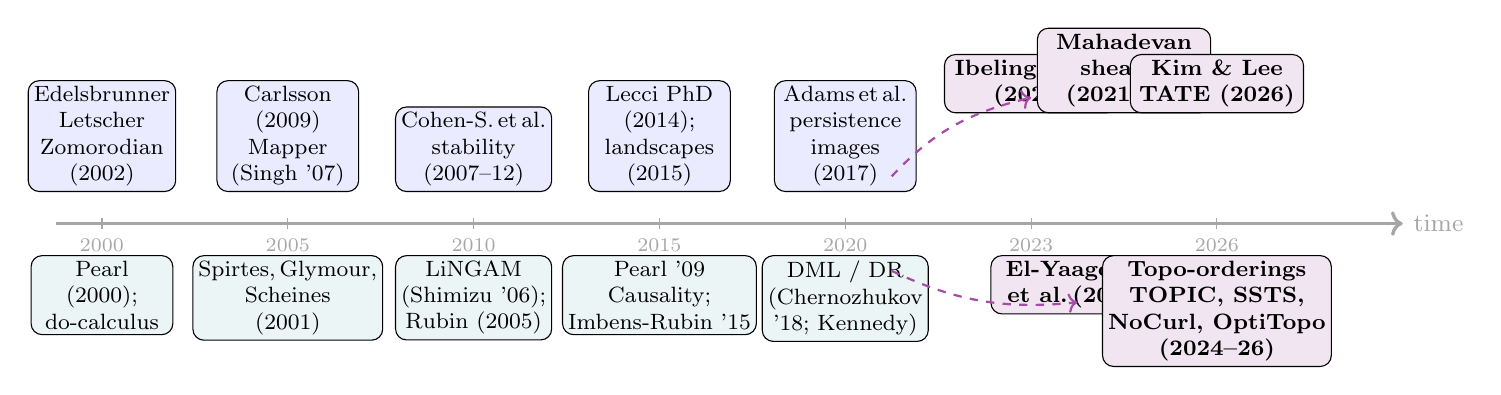
\begin{tikzpicture}[font=\footnotesize,
    yearnode/.style={draw, rounded corners, fill=blue!8, inner sep=2pt,
                     minimum width=18mm, align=center},
    cinode/.style={draw, rounded corners, fill=teal!8, inner sep=2pt,
                   minimum width=18mm, align=center},
    bridge/.style={draw, rounded corners, fill=violet!10, inner sep=2pt,
                   minimum width=22mm, align=center, font=\footnotesize\bfseries},
    xscale=1.18]
\draw[->, very thick, gray!70] (-0.5, 0) -- (14, 0)
  node[right, font=\small] {time};
\foreach \x/\y in {0/2000,2/2005,4/2010,6/2015,8/2020,10/2023,12/2026}{
  \draw[gray!70] (\x,-2pt) -- (\x,2pt) node[below=4pt, font=\scriptsize] {\y};
}
\node[yearnode, anchor=south] at (0,0.4)
  {Edelsbrunner\\Letscher\\Zomorodian\\(2002)};
\node[yearnode, anchor=south] at (2,0.4)
  {Carlsson\\(2009)\\Mapper\\(Singh '07)};
\node[yearnode, anchor=south] at (4,0.4)
  {Cohen-S.\,et\,al.\\stability\\(2007--12)};
\node[yearnode, anchor=south] at (6,0.4)
  {Lecci PhD\\(2014);\\landscapes\\(2015)};
\node[yearnode, anchor=south] at (8,0.4)
  {Adams\,et\,al.\\persistence\\images\\(2017)};

\node[cinode, anchor=north] at (0,-0.4)
  {Pearl\\(2000);\\do-calculus};
\node[cinode, anchor=north] at (2,-0.4)
  {Spirtes,\,Glymour,\\Scheines\\(2001)};
\node[cinode, anchor=north] at (4,-0.4)
  {LiNGAM\\(Shimizu '06);\\Rubin (2005)};
\node[cinode, anchor=north] at (6,-0.4)
  {Pearl '09\\Causality;\\Imbens-Rubin '15};
\node[cinode, anchor=north] at (8,-0.4)
  {DML / DR\\(Chernozhukov\\'18; Kennedy)};

\node[bridge, anchor=south] at (10,1.4)
  {Ibeling-Icard\\(2021)};
\node[bridge, anchor=south] at (11,1.4)
  {Mahadevan\\sheaves\\(2021--25)};
\node[bridge, anchor=south] at (12,1.4)
  {Kim \& Lee\\TATE (2026)};
\node[bridge, anchor=north] at (10.5,-0.4)
  {El-Yaagoubi\\et al.\,(2023)};
\node[bridge, anchor=north] at (12,-0.4)
  {Topo-orderings\\TOPIC, SSTS,\\NoCurl, OptiTopo\\(2024--26)};

\draw[->, dashed, thick, violet!70] (8.5,0.6) to[bend left=18] (10,1.6);
\draw[->, dashed, thick, violet!70] (8.5,-0.6) to[bend right=18] (10.5,-1.0);
\end{tikzpicture}
\caption{Parallel development of TDA (upper band, blue) and causal
inference (lower band, teal) with emerging bridges (violet) in the
2020s. Until $\sim$2020 the two communities developed largely
independently---TDA building from persistence and stability towards a
statistical-inference programme \citep{edelsbrunner2002topological,
carlsson2009topology,cohen2007stability,lecci2014statistical,
adams2017persistence}, while causal inference matured under the Pearl
and Rubin programmes and absorbed double-machine-learning
\citep{pearl2009causality,imbens2015causal,chernozhukov2018double}.
The bridge papers of 2021--2026---topology on the space of SCMs
\citep{ibeling2021topological}, sheaf-theoretic causal calculi
\citep{mahadevan2025sheaf}, topological treatment effects
\citep{kim2026topological}, simulation-based TDA inference for
multivariate time series \citep{elyaagoubi2023statistical}, and
topological-ordering algorithms for causal discovery
\citep{tran2024constraining,xu2025information,nocurl2024,
wu2026optimization}---together delineate the TCDA programme.}
\label{fig:timeline}
\end{figure}


\subsection{Early connections (2015--2019)}\label{sec:lit_early}

The pre-2020 period saw TDA and causal inference develop largely
independently. Three threads, however, foreshadow TCDA: the maturation
of statistical TDA, the rise of topological approaches in
causal-adjacent applications (brain networks, dynamical systems), and
isolated calls for category-theoretic foundations on both sides.

\paragraph{Statistical TDA matures.}
By 2014, the date of \citet{lecci2014statistical}'s PhD thesis-scale
treatise, persistent homology had moved from algebraic topology and
computational geometry into the statistical mainstream. Foundational
algorithmic work \citep{edelsbrunner2002topological,zomorodian2005topology,
zomorodian2005computing} was complemented by a wave of inferential
results: confidence sets for persistence diagrams via the bottleneck
bootstrap \citep{fasy2014confidence,chazal2013bootstrap}; rates of
convergence for the persistent homology of samples
\citep{chaudhuri2010rates,chazal2015optimal}; Banach-space-valued
landscapes that admit a functional central limit theorem
\citep{bubenik2015statistical,chazal2014stochastic,lecci2014statistical};
and probability distributions on the space of diagrams \citep{mileyko2011probability,
turner2014frechet}. \citet{lecci2014statistical} is the most
comprehensive PhD-thesis-scale synthesis of this material; the
inferential machinery it organises---confidence sets, hypothesis tests,
bootstrap, rates---is the statistical scaffolding that any subsequent
TCDA estimator inherits. The introduction of persistence images
\citep{adams2017persistence}, PerLay neural layers
\citep{carriere2020perslay}, and PLLay \citep{kim2020pllay} closed the
gap towards machine-learning workflows, and stability arguments for
the silhouette \citep{chazal2014stochastic} pre-figured the
silhouette-based causal contrast of \citet{kim2026topological}.

\paragraph{Topological brain networks: causal-adjacent but not causal.}
Network neuroscience absorbed TDA early. The Bullmore-Sporns programme
\citep{bullmore2009complex,sporns2013structure,bassett2009human} cast
brain connectivity as a graph, and TDA naturally lifted the discussion
from graphs to higher-order simplicial structures
\citep{sizemore2018cliques,sizemore2019importance}. Cliques and cavities
in the human connectome were shown to organise functional integration
and segregation
\citep{sizemore2018cliques}; small-world propensity was
re-cast as a topological invariant \citep{muldoon2016small}; and trends
in topological summaries of EEG/MEG across cognitive states began to
serve as quantitative biomarkers \citep{fathian2022trend,
gorrostieta2018time}. None of this work was framed in causal terms.
\citet{friston2011functional}'s functional and effective connectivity
agenda was the closest causal counterpart, but it operated in a
parametric (state-space, DCM) framework that did not interact with
topology. The seeds of D1 (TCDA for time-series causality) and C1
(Betti numbers as causal explanation) of \Cref{sec:framework} are here
visible in embryonic form.

\paragraph{TDA for time series and dynamical systems.}
The other natural site of TDA-causality interaction is dynamical
systems: cycles in $\PHk{1}$ of a Takens reconstruction correspond to
recurrent or periodic behaviour. \citet{chung2009persistence,
pachauri2011topology} applied persistence to medical-image time series;
\citet{umeda2017time,kim2018time} used PH features for time-series
classification; \citet{gholizadeh2018short} surveyed the field. Stability
of persistence under filtration deformation
\citep{cohen2007stability,chazal2016structure} ensured that the
features used were not noise artefacts. Crucially, these works treated
PH as a \emph{descriptive} statistic; the next step---using PH inside a
causality test---came after 2020 and is reviewed in
\Cref{sec:lit_method}.

\paragraph{Categorical and sheaf-theoretic preludes.}
On the structural side, \citet{spivak2014category,curry2014sheaves,
robinson2014topological,robinson2014hypothesis} developed category-
theoretic and sheaf-theoretic vocabularies for data analysis,
emphasising functoriality and gluing. Independently, Pearl's
\citep{pearl1995causal,pearl2009causality} programme had been re-cast
in terms of categories of structural equation models, and
\citet{galles1998axiomatic} provided axiomatic foundations for
counterfactuals. \citet{henry2020bridging} explicitly argued that
bridging the two would require new structural primitives. None of
these papers connected TDA to causal inference; together they prepared
the categorical vocabulary that the Mahadevan programme would later
deploy.

\paragraph{Causal-inference foundations that TCDA will inherit.}
Concurrent with the TDA timeline, the causal-inference community
consolidated around three programmes: Pearl's structural-causal-models
and do-calculus \citep{pearl1995causal,pearl2009causality,pearl2018book};
Rubin's potential outcomes \citep{rubin1974estimating,rubin2005causal,
imbens2015causal}; and the constraint-based and score-based discovery
algorithms \citep{spirtes2001causation,meek1995strong,peters2014causal,
shimizu2006lingam}. A separate inferential thread on identification
\citep{tian2000probabilities,tian2002general,avin2005identifiability}
established the language in which any TCDA solution must ultimately be
phrased. The doubly-robust efficient-estimation programme
\citep{robins1989probability,chernozhukov2018double,kennedy2016semiparametric}
would, in turn, supply the AIPW machinery that \citet{kim2026topological}
extend to the topological setting in 2026.

The picture by 2019 is clear: both fields are mathematically and
statistically mature; both have begun to be applied to the same
empirical objects (brain networks, time series, cosmological structure);
and yet no formal bridge yet exists. The four seed papers of the field
all appear within the next four years.

\subsection{Methodological advances (2020--2023)}\label{sec:lit_method}

Between 2020 and 2023 the bridge formed. Five sub-threads emerged in
near-simultaneous fashion: (i)~the topology of the space of structural
causal models; (ii)~category-theoretic and sheaf-theoretic causal
calculi; (iii)~topology-based causal discovery via ordering; (iv)~causal
treatment effects defined directly on topological summaries; and
(v)~topological deep learning with explicit causal applications.

\paragraph{The topology of SCMs.}
\citet{ibeling2021topological} is the methodological pivot for Domain B
of \Cref{sec:framework}. The authors equip the space $\mathfrak{M}$ of
structural causal models with a family of topologies that mirror the
Pearl--Bareinboim causal hierarchy: the observational topology refines
to an interventional topology and then to a counterfactual topology.
The central theorem---a topological no-free-lunch result---states that
the subset of $\mathfrak{M}$ on which assumption-free causal inference is
possible is \emph{topologically meagre} (in the sense of Baire). Two
classical traditions converge here. The first is the measure-theoretic
no-free-lunch programme of \citet{oxtoby1971measure,belot2020absolutely};
the second is the topology-of-statistical-verifiability programme of
\citet{dembo1994topological,genin2017topology,genin2018topology,
genin2020statistical,genin2021statistical}, which shows that open sets
in the weak topology correspond to verifiable statistical hypotheses.
\citet{ibeling2021topological} lifts both to the causal hierarchy and
provides accommodation for SCMs over countably-infinite variable sets
via Borel-product topologies. The companion identifiability papers
\citep{ibeling2019open,ibeling2020probabilistic} complete the picture.
For TCDA, the result is foundational: it tells us that the search for a
causal answer in the absence of topological structure on the model
space is a search in a meagre set, and that topology is the right
language for the negative results of the field.

\paragraph{Sheaf and topos foundations.}
A parallel programme, anchored in \citet{mahadevan2021causal,
mahadevan2022universal,mahadevan2025sheaf}, recasts causal inference as
a universal construction in a topos of sheaves over a base category of
contexts. Do-calculus is recovered through the subobject classifier;
identification becomes a sheaf-cohomological obstruction; the standard
exchangeability/positivity/consistency triple is interpreted as
descent conditions. This work realises B3 (functorial causal inference)
of \Cref{sec:framework} and connects it to the broader categorical
data-analysis programme of \citet{spivak2014category,curry2014sheaves,
hajij2023topological,papamarkou2024position}.
The Alexandroff-topology approach of \citet{willig2025alexandroff}
provides a more elementary entry point and recovers parts of the
Ibeling-Icard hierarchy as Alexandroff specialisations.

\paragraph{Topology-based causal discovery: ordering algorithms.}
A different methodological thread takes the ordering of nodes in a
causal DAG to be the primary object and infers it via topological or
information-theoretic means. The score-based ordering of
\citet{rolland2022score} uses the Hessian of the log-density to
extract a topological order under additive-noise assumptions and was
followed by a wave of related work: TOPIC
\citep{tran2024constraining} uses topological-order constraints in a
DAG-learning loss; SSTS \citep{xu2025information} adapts the order to
sequential and stochastic time-series; NoCurl-X
\citep{nocurl2024} uses the Hodge decomposition of a $1$-chain on the
candidate DAG to extract the harmonic (acyclic) component; OptiTopo
\citep{wu2026optimization} optimises over topological orders directly;
CaPS \citep{rolland2022score} originally introduced the score-Jacobian
formulation. Hodge-decomposition methods more generally
\citep{desilva2007coverage} ground the gradient/curl/harmonic split
that we exploit in C2 (persistent cohomology for mediation analysis).
In the language of \Cref{prop:identifiability}, this entire thread
selects a different topological functor $\Tc$ and asks when the
$G \mapsto \Tc(\mathcal{P}_G)$ map is injective on a class of admissible
graphs.

\paragraph{Treatment effects as topological functionals.}
\citet{kim2026topological} is the methodological pivot for Domains A3
and B1. The authors define the \emph{topological average treatment
effect}
\[
  \TATE = W_1\!\bigl(\Dgmk{k}(P^{a=1}),\,\Dgmk{k}(P^{a=0})\bigr)
\]
and a closely related power-weighted-silhouette contrast, develop a
doubly-robust AIPW estimator with a $\sqrt n$-rate under product-rate
nuisance conditions, prove weak-convergence guarantees in the space of
silhouette functions, supply a $W_1$-based stability bound that links
1-Wasserstein perturbations of the diagram to sup-norm perturbations
of the silhouette, and demonstrate the methodology on SARS-CoV-2 CT
scans \citep{soares2020sars} and the GEOM-Drugs molecular-graph
database \citep{axelrod2022geom}. The work is the first to combine all
three ingredients of TCDA in one estimator: a non-Euclidean outcome
space ($\Mc$ = a space of distributions over diagrams), a topological
functor $\Tc = \varphi(\cdot;r)$, and a causal query $\Cc$ with
calibrated uncertainty. \citet{saki2026beyond} extends the topological-
contrast idea ``beyond the silhouette'' to more general functional
summaries; \citet{ballester2026topological} develops complementary
representations; \citet{deepcausalitytopology2026} connects the
construction to deep causal models. The geodesic-ATE programme of
\citet{kurisu2024geodesic} for Riemannian-valued outcomes is a sister
contribution that places non-Euclidean potential outcomes on the same
footing without invoking persistence.

\paragraph{Simulation-based inference and dependence networks.}
\citet{elyaagoubi2023statistical} addresses an under-served methodological
problem: how to evaluate TDA-based inference for multivariate time
series when no ground truth is available. The authors construct a
generative model---mixtures of latent AR(2) processes---that allows
researchers to \emph{prescribe} the number of cycles in the dependence
network, and they use this to test hypotheses about the resulting
$\PHk{1}$. \citet{elyaagoubi2023topological} extends the construction to
asymmetric dependence. Together these papers anchor D1 (time-series
causality) of \Cref{sec:framework} and provide benchmarking
infrastructure that the rest of the field can adopt.

\paragraph{Topological deep learning and topological regularisation.}
A fifth thread brings topology into representation learning. PerLay
\citep{carriere2020perslay} and PLLay \citep{kim2020pllay} are
differentiable persistence layers that allow gradient-based learning
on diagrams; the topological-deep-learning survey of
\citet{hajij2023topological} consolidates the area, and
\citet{papamarkou2024position} argues for its centrality going forward.
\citet{farzam2025topology} uses topological summaries as
regularisers in causal-representation models, demonstrating robustness
under heavy-tailed noise. \citet{xu2021topological} introduces
topological invariants in deep generative models with causal
structure. \citet{guan2025causal} and \citet{ma2025causal} extend
these ideas to causal disentanglement.

The methodological state by 2023 is therefore that every component of
\Cref{def:tcda}---a topological space $\Mc$ of observations, a causal
graph $G$, a topological functor $\Tc$, and a causal query $\Cc$---is
addressable by at least one well-developed line of research. What is
missing is the joint study.

\subsection{Application-driven work (2020--present)}\label{sec:lit_app}

The 2020--present period saw rapid uptake of TDA in scientific
application areas where causal questions are central. We organise the
account by domain.

\paragraph{Healthcare, drug discovery, and biomedicine.}
TDA of biological structure has a long pedigree \citep{kasson2007persistent,
chung2009persistence}, but causal questions became central only
recently. Persistent homology of protein conformations
\citep{kovacev2016using,cang2018integration} identifies binding-site
topology that responds to ligand intervention---an instance of the
TATE-style contrast in \citet{kim2026topological}, who explicitly use
the GEOM-Drugs molecular-graph database \citep{axelrod2022geom} to
demonstrate that ligand-binding induces topological change. CT-image
analysis of SARS-CoV-2 \citep{soares2020sars,iqbal2025classification}
constructs cubical persistent homology from imaging data and feeds the
resulting summary into classification and treatment-effect estimators;
\citet{kim2026topological} use the same dataset as one of two
methodological case studies. Topological feature extraction in tumour
classification \citep{iqbal2025classification} and disease-progression
modelling on cell-type manifolds
\citep{kim2018topological,carlsson2020topological,corcoran2023topological}
exemplifies the C3 (stratified heterogeneity) and D3 (industry
applications) face of \Cref{sec:framework}. A central remaining issue,
which \Cref{sec:research} treats as an open question, is identifiability
when topological biomarkers are derived from imaging modalities subject
to scanner and protocol drift.

\paragraph{Neuroscience and cognitive science.}
The brain-network literature \citep{bullmore2009complex,bassett2009human,
sporns2013structure,muldoon2016small,sizemore2018cliques,
sizemore2019importance,fathian2022trend} is the densest application
site for sub-domain C1 (Betti numbers as causal explanation): a
persistent $1$-cycle in the functional Granger network of a healthy
brain has been linked to re-entrant cortical loops that
disease---epilepsy, Alzheimer's, schizophrenia---perturbs. Spectral and
graphical extensions \citep{ombao2022spectral,gorrostieta2018time}
sharpen the picture. The simulation framework of
\citet{elyaagoubi2023statistical} ties the empirical literature back to
a controlled testbed: researchers can prescribe how many cycles a
generative model produces and check that a TDA discovery method
recovers them.

\paragraph{Climate, cosmology, and Earth science.}
Persistent homology of cosmological density fields
\citep{sousbie2011persistent,vandeweygaert2011alpha,
cisewski2014nonparametric} established the descriptive template for
spatial TDA, and recent applications transfer this template to climate
weather regimes \citep{strommen2025topological,smith2025multiscale,
smith2025harnessing}. The causal questions in this domain---attribution
of an extreme-precipitation event to a Pacific oscillation, attribution
of regime change to anthropogenic forcing---are precisely the
spatiotemporal causal contrasts of sub-domain D2. To date, however, the
TDA and the attribution communities have proceeded largely in parallel;
the explicit TCDA pairing of $(\Mc, G, \Tc, \Cc)$ in climate science is
nascent.

\paragraph{Finance and economics.}
\citet{gidea2018topological,ismail2022early} apply persistent-landscape
analysis to financial time series and demonstrate that
topological summaries serve as early-warning signals of crashes. The
causal content---attribution of a regime change to a triggering market
factor---is implicit in their construction but not formally tested.
\citet{leykam2023topological} review the broader topological-finance
literature.

\paragraph{Time-series and dynamical-system causality.}
\citet{bando2022causal} combine persistent homology of Takens
embeddings with convergent cross mapping to extract dynamical causal
links between coupled oscillators; \citet{harnack2017causal,
gholizadeh2018short} use persistence to augment Granger-type tests.
\citet{krasnovsky2025causal} extends this to multivariate stochastic
systems with structural breaks. The combination directly instantiates
the sub-domain D1 picture: $\Tc = \PHk{1}$ of a Takens embedding;
$G$ = Granger graph; $\Cc$ = a causal hypothesis test.

\paragraph{Materials and physical sciences.}
TDA in materials science \citep{nigmetov2022topological} and topological
photonics \citep{leykam2023topological} pose causal questions about
structure--property relationships. The TCDA tuple here selects
$\Mc = $ a configuration space of atomic structures, $\Tc = \PHk{0,1,2}$
on the Vietoris-Rips filtration of atomic positions, and $\Cc$ a
causal regression of property on structure mediated by topological
features. This is one of the most natural application domains and is
explicitly identified in \Cref{sec:research}.

\subsection{Gaps in the current literature}\label{sec:lit_gaps}

Five gaps recur across the threads surveyed above. Each motivates a
specific open question or research avenue in \Cref{sec:research}.

\paragraph{Absence of a unified framework.}
The five methodological threads of \Cref{sec:lit_method} fix different
corners of the TCDA tuple but do not interact. \citet{ibeling2021topological}
study topology on $\mathfrak{M}$ but not topological summaries of data;
\citet{kim2026topological} study topological summaries of data but treat
$\mathfrak{M}$ as fixed; \citet{mahadevan2025sheaf} build the
categorical scaffolding without explicit persistence-stability
results; \citet{elyaagoubi2023statistical} provide benchmarks without a
universal causal query. Our \Cref{def:tcda} is the proposed unifier.

\paragraph{Computational and software fragmentation.}
TDA libraries (\texttt{Ripser} \citealp{bauer2021ripser};
\texttt{GUDHI} \citealp{gudhi2021}; \texttt{giotto-tda}
\citealp{tauzin2021giotto}) and causal-inference libraries (\texttt{DoWhy},
\texttt{causal-learn}, \texttt{EconML}) do not interoperate; converting
a persistence diagram into a causal-effect estimand requires custom
plumbing. \Cref{sec:research} lists this as Computational Challenge~C3.

\paragraph{Missing benchmark datasets.}
Causal-discovery benchmarks (CMU-CausalDisco, the CausalBench suite of
\citealp{causaldisco2023survey,timeseriescd2023}) do not include
topological structure as a controlled covariate; conversely,
TDA benchmarks do not encode causal mechanisms. The simulation framework
of \citet{elyaagoubi2023statistical} is the closest analogue but is
restricted to time-series dependence networks; a more general TCDA
benchmark suite is one of the most actionable contributions a community
project could make.

\paragraph{Theoretical disconnect between functorial and methodological threads.}
The Mahadevan sheaf programme \citep{mahadevan2021causal,
mahadevan2022universal,mahadevan2025sheaf} has not yet been used to
analyse the AIPW estimator of \citet{kim2026topological}; conversely,
the Kim-Lee stability theorem has not been re-derived as a
sheaf-cohomological obstruction. The two halves of the field speak
different languages and the dictionary remains to be written. Several
open questions in \Cref{sec:research} (Q3, Q4, Q7) target precisely
this disconnect.

\paragraph{Absence of formal causal interpretation for topological features.}
The brain-network and finance literatures freely use phrases like
``a 1-cycle indicates a feedback loop'' \citep{sizemore2018cliques,
elyaagoubi2023statistical} or ``a persistent crash signature
identifies a regime shift'' \citep{gidea2018topological,
ismail2022early}, but in neither case is the causal interpretation
formally tied to an intervention. Sub-domain C1 of \Cref{sec:framework}
exists precisely because the field has not yet articulated a principled
language for assigning causal semantics to topological features.
\Cref{sec:research} formalises this as Open Question Q5.

\medskip
The methodological building blocks of TCDA are therefore in place; what
the field lacks is the joint formulation, the calibrated estimators,
the interoperable software, the benchmark suites, and the explicit
causal interpretive overlay on topological features.
\Cref{sec:case_studies,sec:research} take these gaps as the starting
point for the agenda we propose.
}{}
\IfFileExists{sections/case_studies.tex}{\section{Case Studies and Proof-of-Concept Synergies}\label{sec:case_studies}

The case studies in this section are intended to demonstrate that the
TCDA tuple of \Cref{def:tcda} is not an empty abstraction: in each of
five concrete settings we can write down the four components
$(\Mc, G, \Tc, \Cc)$ explicitly, locate the example in the taxonomy of
\Cref{fig:taxonomy}, and indicate which parts are already established in
the literature versus which constitute the gaps formalised in
\Cref{sec:research}. The five cases were chosen to (i)~cover all four
top-level domains A--D of the taxonomy, (ii)~engage each of the four
seed works of the field---\citet{ibeling2021topological,
kim2026topological,lecci2014statistical,elyaagoubi2023statistical}---in
at least one case study, and (iii)~span what we expect to be the most
active sites of near-term TCDA research: biomedical imaging and
molecular structure (\Cref{sec:cs_tate}), multivariate brain time series
(\Cref{sec:cs_cycles}), latent-variable confounding diagnostics
(\Cref{sec:cs_confounding}), Mapper-based causal abstraction with
calibrated uncertainty (\Cref{sec:cs_mapper}), and spatiotemporal
climate attribution (\Cref{sec:cs_climate}). \Cref{tab:cs_summary}
summarises the mapping back to the taxonomy.

\subsection{Case Study 1: Topological average treatment effects on
biomedical imaging and molecular structure}\label{sec:cs_tate}

\paragraph{Setting.}
Modern biomedical imaging and computational chemistry deliver
non-Euclidean, high-dimensional outcome data---cubical CT volumes,
volumetric MR scans, three-dimensional molecular point clouds---on
which the classical ATE of \cref{eq:ate} is ill-posed because the
outcome is not a scalar but a shape \citep{soares2020sars,
axelrod2022geom,iqbal2025classification,carlsson2020topological}. The
treatment effect of interest is a contrast between two shape
distributions, not between two means. The first complete TCDA solution
to this problem is the topological average treatment effect of
\citet{kim2026topological}.

\paragraph{TCDA instantiation.}
We instantiate \Cref{def:tcda} as follows. (i)~$\Mc$ is the space of
imaging or molecular outcomes, equipped with a natural ambient metric:
the Hausdorff or Wasserstein distance on $\R^3$ point clouds for
molecular data, the $L^\infty$ pixel distance for cubical images.
(ii)~$G$ is a small ``treatment-to-outcome'' DAG with a binary
treatment $A \in \{0,1\}$ (e.g.\ COVID-positive versus
COVID-negative; ligand-bound versus apo conformation), pre-treatment
covariates $X$ (age, sex, scanner protocol, molecular descriptors),
and the shape-valued outcome $Y \in \Mc$. (iii)~$\Tc$ is composition of
two stable functors: persistent homology
$\PHk{k}$---cubical for images \citep{kaczynski2004computational},
Vietoris--Rips for molecular point clouds---followed by the power-
weighted silhouette $\varphi(\cdot; D, r)$ of \cref{eq:silhouette}.
By \Cref{lem:silhouette_stability}, $\Tc$ is Lipschitz from
$(\mathcal{P}(\Mc), W_1)$ into $L^\infty(T)$. (iv)~$\Cc$ is the
\emph{topological average treatment effect}
\begin{equation}
  \TATE \;=\; \E\bigl[\varphi(\cdot;\,\Tc(Y^1),r)\bigr]
              \;-\; \E\bigl[\varphi(\cdot;\,\Tc(Y^0),r)\bigr],
  \label{eq:tate_silhouette}
\end{equation}
together with the Wasserstein contrast
$W_1(\Dgmk{k}(P^1),\Dgmk{k}(P^0))$ on the underlying diagrams.

\paragraph{Estimation and inference.}
Under the standard identifying assumptions (C1)--(C3) of
\Cref{sec:prelim_ci}, \citet{kim2026topological} construct a doubly-
robust augmented inverse-probability-weighting estimator for
\cref{eq:tate_silhouette} in which the outcome nuisance is a
function-on-vector regression of $\varphi(\cdot; \Tc(Y), r)$ on
$(X,A)$ and the propensity nuisance is $\widehat\pi(x) = \widehat\Prob(A=1\mid X = x)$.
Under product-rate nuisance conditions the estimator achieves a
$\sqrt n$ functional rate in $L^\infty(T)$ and admits a tight
weak-convergence limit, from which a level-$\alpha$ test of
$H_0 : W_1(\Dgmk{k}(P^1),\Dgmk{k}(P^0)) = 0$ is read off. The
statistical scaffolding inherits directly from
\citet{lecci2014statistical}'s programme of confidence sets and
bootstrap procedures for persistence diagrams, landscapes, and
silhouettes; without this scaffolding, the TCDA estimator would deliver
a point estimate but no uncertainty.

\paragraph{Stability.}
The estimator inherits the quantitative robustness of persistent
homology via \Cref{prop:stability-transfer}: a Hausdorff perturbation
of the support of $P^a$ translates into an $L^\infty$ perturbation of
the estimated silhouette TATE, with an explicit constant tracking the
silhouette weight $r$. This is the concrete payoff of Domain B1:
where classical AIPW estimators are sensitive to imaging artefacts and
scanner drift, the topological AIPW estimator is provably robust to
small Hausdorff perturbations of the support.

\paragraph{Why this case study matters and what remains open.}
The case study completely populates one ``corner'' of the TCDA
taxonomy---sub-domains A3 and B1, with applications in D3---and is the
clearest existence proof that the framework is non-vacuous: a
non-Euclidean outcome that previously admitted only descriptive TDA
now admits a calibrated, doubly-robust causal estimator. Remaining
gaps targeted in \Cref{sec:research} include the scaling of
$\PHk{k}$ to volumetric three-dimensional inputs, transportability of
the estimator across imaging protocols (a positivity issue), and the
extension of the construction to non-binary or continuous treatments.

\subsection{Case Study 2: Cycle-based causal discovery in
multivariate dependence networks}\label{sec:cs_cycles}

\paragraph{Setting.}
Multivariate time-series data---neural recordings, financial returns,
climate indices---admit a natural \emph{dependence network} whose edges
are weighted by pairwise statistical dependence (mutual information,
partial coherence, transfer entropy). Causal questions on these
networks concern the presence and direction of feedback loops:
re-entrant cortical loops in EEG \citep{sizemore2018cliques,
elyaagoubi2023statistical}, contagion cycles in financial markets
\citep{gidea2018topological,ismail2022early}, oceanic--atmospheric
teleconnections in climate \citep{strommen2025topological}. Persistent
homology of the dependence network in homology degree~$1$ is the
natural detector of such loops.

\paragraph{TCDA instantiation.}
We set (i)~$\Mc$ = the space of multivariate windowed time series in
$\R^d$ with the supremum-distance topology; (ii)~$G$ = a directed
Granger or transfer-entropy graph encoding lagged causal influence
among the $d$ variables; (iii)~$\Tc$ = the composition ``windowed
dependence network'' $\to$ ``filtration by edge weight'' $\to$
$\PHk{1}$, optionally smoothed by the silhouette of
\cref{eq:silhouette}; (iv)~$\Cc$ = a hypothesis test on the number of
persistent $1$-cycles in $\Dgmk{1}$, or---more ambitiously---a recovery
test for the cycle structure of $G$ from $\Dgmk{1}$. The construction
is exactly the one analysed in \citet{elyaagoubi2023statistical}, whose
mixture of latent AR(2) processes allows researchers to \emph{prescribe}
the number of cycles in the network and so to evaluate $\Tc$-based
discovery procedures against ground truth.

\paragraph{Inference and benchmark.}
\citet{elyaagoubi2023statistical} construct simulation-based confidence
regions for $\PHk{1}$ of the dependence network and use them to test
hypotheses about cycle count. The companion work
\citet{elyaagoubi2023topological} extends the construction to
asymmetric dependence and so to genuinely directed Granger graphs. The
case study realises sub-domains A1 (PH for causal structure learning),
C1 (Betti numbers as causal explanation), and D1 (time-series
causality) of \Cref{sec:framework} in a single, fully executable
pipeline. \citet{bando2022causal,harnack2017causal,gholizadeh2018short,
krasnovsky2025causal} pursue closely related strategies for dynamical
causal links via PH of Takens embeddings, providing a complementary
source of empirical evidence.

\paragraph{From a cycle to a causal mechanism.}
Sub-domain C1 raises the harder question: when does a persistent
$1$-cycle deserve the label ``causal feedback loop'' rather than the
weaker label ``cyclic correlation pattern''? The dependence-network
construction does not, on its own, supply directionality. A natural
answer, partial but concrete, is provided by \Cref{prop:identifiability}
specialised to the dependence-network functor $\Tc$: if the assignment
$G \mapsto \Tc(\mathcal{P}_G)$ is injective on a class of admissible
graphs (e.g.\ acyclic Granger graphs with non-Gaussian innovations,
in which case classical identifiability via the LiNGAM family applies
\citep{shimizu2006lingam}), then $\PHk{1}$-based discovery is
identifying. Where this injectivity condition fails---e.g.\ for two
distinct cyclic graphs that yield the same windowed dependence
network---the $1$-cycle is a \emph{joint} causal pattern of an
equivalence class of graphs, and downstream identification requires
auxiliary assumptions. The simulation framework of
\citet{elyaagoubi2023statistical} makes both successful and unsuccessful
cases controllable in the laboratory, and we list the
characterisation of injectivity as an explicit open avenue in
\Cref{sec:research}.

\paragraph{Why this case study matters and what remains open.}
The case study shows that an existing TDA benchmark is essentially a
TCDA benchmark in waiting: equipping the dependence-network filtration
with an explicit causal graph $G$ converts the topological cycle
detector into a topological causal-discovery procedure, with calibrated
uncertainty inherited from \citet{lecci2014statistical}'s programme.
The remaining methodological gap is the formal identifiability theory
that would convert the construction from a benchmark-validated heuristic
into a procedure with deductive guarantees on real (non-simulated)
multivariate time series.

\subsection{Case Study 3: Confounding diagnostics via persistent
residual topology}\label{sec:cs_confounding}

\paragraph{Setting.}
Suppose an analyst posits a causal graph $G$ over an observed set of
variables and fits the corresponding SCM. Under correct specification
the residuals are independent of the predicted endogenous variables
and---crucially for TCDA---their joint support carries no topological
information beyond Euclidean noise. When an unobserved confounder
$U$ acts on two or more observed variables along an unobserved orbit,
the residual support inherits a persistent low-dimensional topology
that no orientation of edges within $G$ can explain. This observation
is the basis of \emph{topological confounding diagnostics}
(sub-domain B2 of \Cref{sec:framework}) and connects, via
\citet{ibeling2021topological}, to the topological no-free-lunch
theorem of the field.

\paragraph{TCDA instantiation.}
(i)~$\Mc$ = the residual space of a fitted SCM, viewed as a point cloud
in $\R^{|V|}$; (ii)~$G$ = the analyst's hypothesised graph, treated as
a null hypothesis; (iii)~$\Tc$ = $\PHk{1}$ of the Vietoris--Rips
filtration of the residual cloud, with bootstrap confidence sets
\citep{fasy2014confidence,chazal2013bootstrap}; (iv)~$\Cc$ = a test of
the null hypothesis ``the persistent $1$-classes of $\Tc$ have
lifetimes consistent with white-noise residuals.''

\paragraph{Worked example: the circular confounder.}
Let $U$ be uniformly distributed on the unit circle $S^1$ and define
$X = \cos U + \epsilon_X$ and $Y = \sin U + \epsilon_Y$ with
$\epsilon_X, \epsilon_Y$ small, independent, mean-zero noise. An
analyst who assumes no edge $X \to Y$ and no confounder will correctly
estimate $\widehat{\ATE}(X \to Y) \approx 0$, since on average $X$
carries no information about $Y$. The same analyst, however, will
discover a persistent $1$-cycle in $\Dgmk{1}$ of the $(X,Y)$ residuals
whose lifetime exceeds any plausible noise band, signalling the action
of $U$. Formally:

\begin{proposition}[Topological confounding signature]
\label{prop:confounding_signature}
Let $U$ be a continuous random variable supported on a topological
space $\mathcal{U}$ with non-trivial $H_1(\mathcal{U};\R) \neq 0$, and
let $X_v = f_v(U,\epsilon_v)$ for $v \in V$ with $f_v$ continuous and
$\epsilon_v$ Gaussian and independent of $U$. Suppose the analyst's
hypothesised graph $G$ omits $U$ and is otherwise correct. Then the
limit support of the joint residuals admits a continuous surjection
onto $\mathcal{U}$, and the persistent $\PHk{1}$ of any sufficiently
fine Vietoris--Rips filtration of the residuals contains at least one
class whose expected lifetime is bounded away from zero uniformly in
the noise scale.
\end{proposition}

\begin{proof}[Sketch]
By the continuous-mapping theorem and the assumed continuity of each
$f_v$, the image of $U$ under $v \mapsto X_v$ is a continuous
surjection $\mathcal{U} \to \mathrm{supp}(P^{X})$. The corresponding
homology map $H_1(\mathcal{U}) \to H_1(\mathrm{supp}(P^X))$ is
non-trivial whenever the $(f_v)$ collectively are not homotopic to a
constant, which is generic. The stability theorem
(\cref{eq:stability}) ensures that the corresponding cycle persists in
the empirical $\PHk{1}$ of finite samples, with lifetime bounded below
by the homological diameter of $\mathcal{U}$. Full details, including
the rate at which the lifetime concentrates, follow the stability
arguments of \citet{cohen2007stability,chazal2016structure}.
\end{proof}

\paragraph{Discussion: detection is not identification.}
\Cref{prop:confounding_signature} is one-sided: a persistent residual
$1$-cycle is consistent with confounding but does not, on its own,
recover $U$ or even identify the variables it acts on. This asymmetry
is exactly the content of the topological causal hierarchy theorem of
\citet{ibeling2021topological}: the set of SCMs admitting
assumption-free identification of $P(y\mid \doop(x))$ is topologically
meagre, so almost any SCM carries residual topological structure that
\emph{flags} confounding but cannot \emph{certify} its absence. The
sheaf-theoretic programme of \citet{mahadevan2021causal,
mahadevan2022universal,mahadevan2025sheaf} provides a complementary
reading in which the residual cycle is interpreted as a non-trivial
class in a sheaf-cohomology obstruction to identification; this is
the natural home of sub-domain B3.

\paragraph{Why this case study matters and what remains open.}
The case study converts an existing TDA descriptor---persistent
$1$-cycles of a point cloud---into a diagnostic that is logically
linked to a causal property (residual confounding) via
\Cref{prop:confounding_signature}, and shows that the limits of the
diagnostic are precisely those identified in
\citet{ibeling2021topological}'s meagre-set theorem. Operationalising
the test on real data---calibrating the lifetime threshold against
noise, controlling for nuisance topology induced by sampling, and
extending to higher-dimensional confounders with $H_k(\mathcal{U}) \neq 0$
for $k \ge 2$---are the principal methodological gaps.

\subsection{Case Study 4: Mapper-based causal abstraction with
calibrated uncertainty}\label{sec:cs_mapper}

\paragraph{Setting.}
Many causal questions in medicine and the social sciences concern
\emph{regimes}: disease subtypes, treatment-responder strata, market
phases. Regimes are typically not pre-specified by covariates but emerge
from the geometry of the data. The Mapper algorithm
\citep{singh2007mapper,carriere2018statistical,dlotko2019ball,
madukpe2026mapper} produces a topological abstraction of a
high-dimensional data set into a simplicial complex whose nodes are
clusters of level sets of a chosen filter $f$; we propose that Mapper
abstractions are the natural carrier of a regime-conditional causal
estimand, and that \citet{lecci2014statistical}'s bootstrap-confidence
programme delivers the calibrated uncertainty that regulated industries
require.

\paragraph{TCDA instantiation.}
(i)~$\Mc$ = a high-dimensional feature space of patient (or asset)
descriptors. (ii)~$G$ = a coarse-grained DAG over Mapper nodes
representing regimes and edges representing admissible transitions or
treatment effects between regimes; we assume $G$ is acyclic for
identification, while permitting cycles inside the data Mapper graph
itself. (iii)~$\Tc = \Map_f$ with a filter $f$ chosen to align with the
causal mechanism (disease severity, time-to-event, an exposure score).
(iv)~$\Cc$ = a stratum-conditional ATE, defined for each Mapper node
$\alpha$ by
\begin{equation}
  \CATE(\alpha) \;=\; \E\bigl[\,Y^1 - Y^0 \;\big|\; X \in \alpha\,\bigr],
  \label{eq:cate_mapper}
\end{equation}
together with its uncertainty.

\paragraph{Bootstrap confidence sets for the abstraction.}
The statistical-TDA programme of \citet{lecci2014statistical} supplies
the inferential scaffolding for $\Tc$ via the bottleneck bootstrap of
\citet{fasy2014confidence,chazal2013bootstrap}: a confidence band
$\mathcal{B}_n^{1-\alpha}$ around the empirical persistence diagram of
the Mapper complex covers the population diagram with probability at
least $1 - \alpha$. Translating $\mathcal{B}_n^{1-\alpha}$ into
uncertainty for \cref{eq:cate_mapper} proceeds in two stages. First,
we bootstrap the Mapper graph to obtain a posterior over regime
boundaries, propagating the cluster-membership uncertainty to each
patient or asset. Second, we use the resulting node-level posterior
weights as inputs to a regime-conditional AIPW estimator. The
combination delivers, for each Mapper node $\alpha$, a point estimate
$\widehat\CATE(\alpha)$ and a confidence interval that accounts for
both the topological (regime-assignment) and statistical
(treatment-effect) sources of uncertainty.

\paragraph{Connection to stratified-space causal heterogeneity.}
The Mapper output is a stratified topological abstraction: nodes are
$0$-strata, edges are $1$-strata, and higher simplices encode
higher-order regime overlaps. The theory of stratified spaces
\citep{hughes2004stratified,banagl2007topological,chazal2013persistence}
is exactly the right language for causal effects that vary across such
strata---sub-domain C3 of \Cref{sec:framework}. The bootstrap pipeline
sketched above is therefore a concrete instantiation of Domains A2,
B1, and C3 simultaneously.

\paragraph{Why this case study matters and what remains open.}
The case study addresses a critique frequently levelled at
Mapper-based causal claims in healthcare and finance: the abstraction
is descriptive, not inferential, and conveys no notion of statistical
confidence. \citet{lecci2014statistical}'s programme dissolves the
critique, provided the abstraction is treated as a TCDA functor. The
open methodological question is the design of filter functions $f$
that are simultaneously (i)~causally informative---i.e.\ aligned with
the mechanism of interest---and (ii)~statistically well-behaved under
the bootstrap. We list this as a research avenue in \Cref{sec:research}.

\subsection{Case Study 5: Spatiotemporal causal attribution via
cubical persistent homology}\label{sec:cs_climate}

\paragraph{Setting.}
Climate-event attribution asks whether a specific extreme event would
have occurred in a counterfactual climate without anthropogenic
forcing. Conventional attribution operates on scalar summaries of the
event (return period, intensity) and so is blind to the spatial
structure of the extreme. Cubical persistent homology of the climate
field captures that structure---the number of connected hot regions,
the topology of pressure ridges, the persistence of low-pressure
cells---and so naturally supports a topological notion of attribution
\citep{strommen2025topological,smith2025multiscale,smith2025harnessing}.

\paragraph{TCDA instantiation.}
(i)~$\Mc$ = the space of gridded scalar fields on $\R^2 \times [0,T]$
(daily precipitation, surface temperature, geopotential height), with
the $L^\infty$ pixel-wise distance. (ii)~$G$ = a coarse climate causal
graph linking forcing (anthropogenic emissions, sea-surface
temperature anomalies, modes of variability) to the spatial event
field; the binary attribution treatment is ``factual climate'' versus
``counterfactual climate'' produced by a model ensemble.
(iii)~$\Tc$ = cubical $\PHk{k}$ for $k \in \{0,1\}$ of the sublevel
sets, with optional silhouette smoothing. (iv)~$\Cc$ = a
counterfactual contrast between persistence diagrams,
\begin{equation}
  \Cc_{\mathrm{attr}}
  \;=\; W_1\!\bigl(\Dgmk{k}(P^{\text{fact}}),
                   \Dgmk{k}(P^{\text{cf}})\bigr),
  \label{eq:climate_contrast}
\end{equation}
or its silhouette functional analogue analogous to
\cref{eq:tate_silhouette}.

\paragraph{The descriptive precedent and the causal upgrade.}
The cosmology literature \citep{sousbie2011persistent,
vandeweygaert2011alpha,cisewski2014nonparametric} provides the mature
descriptive template: persistence diagrams of cosmological density
fields characterise the cosmic web, and bootstrap confidence sets
on those diagrams supply calibrated descriptive uncertainty. The TCDA
upgrade is straightforward in principle: replace cosmology's
``observed universe vs.\ simulated universe'' contrast by climate's
``factual climate vs.\ counterfactual climate'' contrast, and apply
the AIPW machinery of \citet{kim2026topological} treating each ensemble
member as a sample from the relevant interventional distribution. The
stability transfer of \Cref{prop:stability-transfer} controls the
sensitivity of \cref{eq:climate_contrast} to grid resolution and to
the small Hausdorff-scale perturbations that arise from regridding,
bias correction, and interpolation.

\paragraph{Why this case study matters and what remains open.}
The case study realises sub-domains D2 (spatiotemporal causality) and
B1 (stability of causal estimates) of \Cref{sec:framework} on a
high-impact application. The principal remaining gap is identifiability
of \cref{eq:climate_contrast} under unobserved natural variability:
a coupled-model ensemble approximates the counterfactual distribution
but does not eliminate the latent low-frequency oscillations that act
as confounders. \Cref{prop:confounding_signature} suggests a built-in
diagnostic: a persistent $1$-cycle in the residual climate field
\emph{after} adjustment for the assumed forcing covariates would
flag that some mode of variability has not been accounted for, and so
the attribution estimate carries the residual topology of the
unidentified causal structure. Climate TCDA is therefore both a
showcase application and a stress test of the framework: its
methodological success will depend on whether the diagnostics of
sub-domain B2 can be deployed in concert with the estimators of
sub-domains A3 and B1.

\subsection{Synthesis: case studies and the taxonomy}\label{sec:cs_synthesis}

\Cref{tab:cs_summary} collects the case studies of this section, the
seed and bridge works that anchor each, and the taxonomy nodes of
\Cref{fig:taxonomy} that the case study populates.

\begin{table}[t]
\centering
\caption{Case studies and their place in the TCDA taxonomy of
\Cref{fig:taxonomy}. Each case study instantiates the TCDA tuple
$(\Mc, G, \Tc, \Cc)$ of \Cref{def:tcda} in a specific applied or
theoretical setting, engages one or more of the four seed works of
the field, and populates one or more sub-domains of the taxonomy.}
\label{tab:cs_summary}
\begin{tabular}{@{}lp{0.36\linewidth}p{0.28\linewidth}p{0.16\linewidth}@{}}
\toprule
\S & Case study & Seed and bridge works & Taxonomy node(s) \\
\midrule
\ref{sec:cs_tate}        & Topological ATE on biomedical imaging
                         & \citet{kim2026topological,
                                  lecci2014statistical,
                                  soares2020sars,axelrod2022geom}
                         & A3, B1, D3 \\
\ref{sec:cs_cycles}      & Cycle-based discovery in dependence networks
                         & \citet{elyaagoubi2023statistical,
                                  elyaagoubi2023topological,
                                  bando2022causal}
                         & A1, C1, D1 \\
\ref{sec:cs_confounding} & Confounding diagnostics via residual PH
                         & \citet{ibeling2021topological,
                                  mahadevan2025sheaf,
                                  fasy2014confidence}
                         & B2, B3 \\
\ref{sec:cs_mapper}      & Mapper abstractions with calibrated uncertainty
                         & \citet{lecci2014statistical,
                                  singh2007mapper,
                                  carriere2018statistical}
                         & A2, B1, C3 \\
\ref{sec:cs_climate}     & Spatiotemporal climate attribution
                         & \citet{kim2026topological,
                                  sousbie2011persistent,
                                  strommen2025topological}
                         & D2, B1, B2 \\
\bottomrule
\end{tabular}
\end{table}

Three observations emerge from the synthesis. First, every cell of the
TCDA tuple $(\Mc, G, \Tc, \Cc)$ is exercised non-trivially in at least
one case study: $\Mc$ ranges over image spaces, time-series spaces,
residual spaces, feature spaces, and climate-field spaces; $G$ ranges
from simple treatment-to-outcome DAGs through dependence networks to
coarse-grained regime graphs; $\Tc$ ranges over $\PHk{k}$ in
Vietoris--Rips, cubical, dependence-network, and Mapper forms; and
$\Cc$ ranges over Wasserstein contrasts, silhouette ATEs, hypothesis
tests, and stratum-conditional CATEs. The expressive scope of
\Cref{def:tcda} is therefore borne out empirically.

Second, the four seed works each anchor at least one case study, but no
single seed work anchors more than two: the field is not the work of any
one author or group, and a serious TCDA programme must draw on all four
threads in parallel. The relative position of the seed works in the
case-study landscape---\citet{kim2026topological} as the estimator
champion, \citet{ibeling2021topological} as the no-free-lunch theorist,
\citet{lecci2014statistical} as the statistical infrastructure, and
\citet{elyaagoubi2023statistical} as the benchmark architect---is
exactly the four-cornered division of labour anticipated in
\Cref{sec:framework}.

Third, every case study identifies a concrete remaining gap that we
take up explicitly in \Cref{sec:research}: scaling, transportability,
identifiability, filter design, and identification under unobserved
variability. The case studies are therefore not endpoints but launch
pads, and the agenda of \Cref{sec:research} is calibrated against them.
}{}
\IfFileExists{sections/research_agenda.tex}{\section{Research Agenda and Open Questions}\label{sec:research}

We close the technical part of the paper with a structured research
agenda. The agenda is calibrated against the gaps identified in
\Cref{sec:lit_gaps} and against the methodological openings left by the
case studies of \Cref{sec:case_studies}, and is organised along five
branches: theoretical open questions (\Cref{sec:research_theory}),
methodological research avenues (\Cref{sec:research_method}),
computational and algorithmic challenges
(\Cref{sec:research_compute}), domain-specific opportunities
(\Cref{sec:research_domains}), and industry- and implementation-facing
problems (\Cref{sec:research_industry}). Eleven formal Open Questions,
fourteen Research Avenues, and four Computational Challenges are
distributed across these branches; \Cref{fig:research_mindmap}
summarises the overall structure, and each item is formulated to be
specific enough to underwrite a self-contained research project or
grant proposal.

\subsection{Theoretical open questions}\label{sec:research_theory}

The theoretical core of TCDA is the formal study of the four-tuple
$(\Mc, G, \Tc, \Cc)$ of \Cref{def:tcda} and of the conditions under
which its components interact coherently. The questions below organise
the agenda along the algebraic, categorical, statistical, and
interpretive axes of that interaction.

\begin{question}[Causal persistent modules]\label{q:causal-modules}
Let $(P_t)_{t \ge 0}$ be a one-parameter family of interventional
distributions induced by a continuously varying intervention $\doop(x_t)$
on an SCM $\Mc$. Define a \emph{causal persistent module}
$M^{\Cc}_\bullet$ as the persistent homology of $(P_t)_{t \ge 0}$ with
respect to a $\Cc$-graded filtration, so that birth and death scales
encode the strength and duration of causal effects. Does
$M^{\Cc}_\bullet$ admit a Crawley--Boevey-type decomposition into
interval modules indexed by causal effects, and if so, do the resulting
intervals coincide with classically identified causal estimands?
\end{question}

A positive answer would give an algebraic invariant of an SCM whose
indecomposables are causal effects, in direct analogy with the way the
indecomposables of an ordinary persistent module are barcode intervals.
The question is open at every level: existence, uniqueness, stability,
and computability.

\begin{question}[Functorial adjoints for TCDA]\label{q:adjoints}
Let $\Tc : \mathbf{SCM} \to \mathbf{Pers}$ be a topological functor in
the sense of \Cref{def:tcda}. Does $\Tc$ admit a left or right adjoint
$\Tc^\sharp : \mathbf{Pers} \to \mathbf{SCM}$, and if so, what causal
quantities does the unit
$\eta : \mathrm{id} \Rightarrow \Tc^\sharp \circ \Tc$ or the counit
$\epsilon : \Tc \circ \Tc^\sharp \Rightarrow \mathrm{id}$ compute?
\end{question}

Adjoints, if they exist, would systematically convert TDA-level data
into the SCM that ``best explains'' it, providing a categorical
foundation for inverse problems in causal discovery. The question
sharpens the sheaf-theoretic programme of \citet{mahadevan2021causal,
mahadevan2022universal,mahadevan2025sheaf} and ties it to the
functorial-data-analysis tradition of \citet{spivak2014category,
curry2014sheaves,hajij2023topological}.

\begin{question}[Causal stability theorem]\label{q:causal-stability}
Let $\Mc_1, \Mc_2$ be SCMs in the weak Ibeling--Icard topology on
$\mathfrak{M}$ and let $\Tc = \PHk{k}$. Suppose
$\dB\bigl(\Tc(p^{\Mc_1}), \Tc(p^{\Mc_2})\bigr) < \epsilon$. What is the
tightest upper bound, as a function of $\epsilon$ and $G$, on
\[
\sup_{x,y} \bigl\lVert P_{\Mc_1}(y \mid \doop(x))
                    - P_{\Mc_2}(y \mid \doop(x)) \bigr\rVert_{\mathrm{TV}}\,?
\]
\end{question}

This is the quantitative completion of \Cref{prop:stability-transfer}:
the proposition shows that any Lipschitz causal functional inherits
robustness from bottleneck stability, but it leaves open the explicit
bound for the central object of Pearl's framework---the interventional
distribution itself. A positive answer would bridge the sheaf
programme \citep{mahadevan2025sheaf} and the AIPW programme
\citep{kim2026topological,chernozhukov2018double} by giving the
``other half'' of the dictionary: not just that diagrams perturb under
data perturbation, but that do-effects perturb under diagram
perturbation.

\begin{question}[Identifiability of $G$ from a topological functor]
\label{q:tcda-identifiability}
For a fixed admissible topological functor $\Tc$ and a class
$\mathcal{G}$ of DAGs, characterise necessary and sufficient
conditions for the assignment $G \mapsto \Tc(\mathcal{P}_G)$ to be
injective on $\mathcal{G}$. In particular: for which classes
$\mathcal{G}$ is $\Tc = \PHk{1}$ of the windowed dependence network of
\citet{elyaagoubi2023statistical} identifying?
\end{question}

\Cref{prop:identifiability} reduces TCDA identifiability to an
injectivity question; \Cref{q:tcda-identifiability} asks for the
algebraic characterisation of that injectivity. The classical
identifiability results for linear non-Gaussian models
\citep{shimizu2006lingam} and for score-based topological orderings
\citep{rolland2022score,tran2024constraining,xu2025information,
nocurl2024,wu2026optimization} are the natural touchstones.

\begin{question}[Causal semantics for persistent cycles]
\label{q:cycle-semantics}
Develop a calculus for assigning a causal label
(\emph{feedback}, \emph{confounding}, \emph{mediation}, \emph{spurious})
to a persistent $1$-cycle in $\Dgmk{1}(\Tc(X))$. Specifically, give
sufficient observational and interventional tests that distinguish a
cycle generated by a directed feedback loop in $G$ from a cycle
generated by an unobserved low-dimensional confounder.
\end{question}

This is the formal language whose absence is identified as a gap in
\Cref{sec:lit_gaps}. \Cref{prop:confounding_signature} supplies a
one-sided test (residual cycle signals possible confounding); the
question asks for the analogous tests for the other three cases and
for the cohomological-charge calculus that would tie them together.

\begin{question}[Persistent cohomology for mediation]
\label{q:cohomology-mediation}
Let $A \to M \to Y$ be a mediation triple with a multidimensional
mediator $M \in \R^d$. Apply the Hodge decomposition
\citep{desilva2007coverage,nocurl2024} to a $1$-chain on the simplicial
complex generated by the empirical distribution of $(A, M, Y)$ and
decompose it into gradient (acyclic), curl (cyclic), and harmonic
(globally non-trivial) components. Does the resulting decomposition
recover the Pearl natural direct/natural indirect effect decomposition
\citep{pearl2009causality}, and, if so, under what regularity
conditions on the mediator distribution?
\end{question}

A positive answer would convert mediation analysis from a parametric
exercise to a cohomological computation; the harmonic component, in
particular, would quantify mediation that no local mediator captures.

\begin{question}[Sheaf-cohomological reading of AIPW stability]
\label{q:sheaf-aipw}
Re-derive the stability bound of \citet[Theorem on silhouette
stability]{kim2026topological} as a sheaf-cohomological obstruction in
the topos of \citet{mahadevan2025sheaf}. Identify the obstruction class
that vanishes if and only if the AIPW estimator on $\Tc$ inherits
$\sqrt n$ rates under product-rate nuisance conditions.
\end{question}

\Cref{q:sheaf-aipw} is the most concrete instance of the
methodological dictionary called for in \Cref{sec:lit_gaps}: the
categorical and the asymptotic-statistical halves of TCDA must speak
the same language before the field can be regarded as mature.

\begin{question}[Functional CLT for TCDA beyond silhouettes]
\label{q:functional-clt}
Establish a functional central limit theorem for AIPW-type estimators
of $\Cc = \E[\Tc(Y^1) - \Tc(Y^0)]$ for general admissible $\Tc$,
including persistence landscapes \citep{bubenik2015statistical},
persistence images \citep{adams2017persistence}, and Euler
characteristic curves. Identify the natural function space and the
covariance structure of the limit.
\end{question}

The silhouette case is settled by \citet{kim2026topological}, but
landscapes, images, and Euler curves carry different smoothness and
sparsity properties and require their own central-limit machinery,
parallel to but distinct from \citet{bubenik2015statistical}'s
functional CLT for landscape means.

\begin{question}[Positivity for non-Euclidean outcomes]
\label{q:positivity-noneuclidean}
Reformulate the positivity assumption (C3) of \Cref{sec:prelim_ci} for
outcomes valued in a non-Euclidean topological space $\Mc$. Is the
classical pointwise overlap condition
$0 < \Prob(A = 1 \mid X) < 1$ sufficient, or is a topological
covering condition---e.g.\ each connected component of $\mathrm{supp}\,P^X$
intersects both treatment arms---also required for the topological
contrasts of \cref{eq:tate_silhouette,eq:climate_contrast} to be
identifiable?
\end{question}

Positivity violations occur silently when the outcome lives on a
manifold or stratified space: a covariate stratum can have positive
probability on one connected component of $\Mc$ and zero on another,
without violating the classical scalar overlap.
\Cref{q:positivity-noneuclidean} asks for the topological refinement
of overlap that detects this.

\begin{question}[Transportability across topological domains]
\label{q:transportability}
Develop a transportability theory \citep{pearl2014external,
bareinboim2020pearls} for TCDA estimators: under what conditions on
$\Tc$, on the imaging or measurement modality, and on the causal
graph $G$ can $\widehat\Cc_n$ estimated on a source domain
$(\Mc^{\mathrm{src}}, G)$ be transported to a target domain
$(\Mc^{\mathrm{tgt}}, G)$ with bounded loss?
\end{question}

The case study of \Cref{sec:cs_tate} motivates the question: the
SARS-CoV-2 CT-scan TATE of \citet{kim2026topological} is evaluated on
a single scanner protocol, and the practical deployment of a TCDA
estimator across heterogeneous clinical sites requires a
transportability calculus.

\begin{question}[Topological do-calculus]\label{q:topo-docalculus}
Develop a topological do-calculus: a set of rewrite rules acting on
persistence diagrams, landscapes, or silhouettes that mirror Pearl's
three do-calculus rules and produce, in the limit, the same
identification answers. Identify the topological analogues of the
three Pearlian conditions (insertion/deletion of observations,
exchanging actions and observations, and insertion/deletion of
actions).
\end{question}

A topological do-calculus would extend the categorical work of
\citet{mahadevan2025sheaf} into a constructive algorithmic procedure,
and would supply the inferential engine that
\Cref{q:tcda-identifiability} demands.

\subsection{Methodological research avenues}\label{sec:research_method}

The methodological agenda translates the theoretical questions of
\Cref{sec:research_theory} into algorithms, estimators, and learning
procedures. We enumerate five core avenues.

\begin{research}[Causal Mapper]\label{r:causal-mapper}
Design a \emph{causal} variant of the Mapper algorithm
\citep{singh2007mapper,carriere2018statistical} whose output is not a
simplicial complex but a partially directed mixed graph (PDMG) over
Mapper nodes, with edge orientations inferred from local conditional
independence tests within each cluster. Provide bootstrap-based
confidence guarantees on the orientation of each edge, building on
\citet{lecci2014statistical}.
\end{research}

The case study of \Cref{sec:cs_mapper} sketches the calibrated-CATE
side of this avenue; \Cref{r:causal-mapper} asks for the algorithmic
upgrade that recovers a graph rather than a complex.

\begin{research}[Persistent causal homotopy]\label{r:causal-homotopy}
Develop a theory of \emph{persistent causal homotopy} for time-varying
causal systems: a two-parameter persistence framework
\citep{carlsson2009theory,lesnick2015interactive} in which one
direction is the topological filtration scale and the other is causal
time, and the bigraded module encodes both the topology of cross-
sectional dependence and its temporal evolution.
\end{research}

\citet{elyaagoubi2023statistical} provide the empirical analogue
(windowed dependence networks); \Cref{r:causal-homotopy} promotes the
analogue to a calibrated bigraded estimator with formal interpretation
in terms of regime changes and causal-structure shifts.

\begin{research}[Topological regularisation for neural causal models]
\label{r:topo-regularisation}
Use topological summaries as regularisers in deep generative causal
models, extending \citet{xu2021topological,farzam2025topology,
guan2025causal,ma2025causal}. The objective is a causal variational
autoencoder whose latent space is constrained to have prescribed
persistent homology, encouraging causally meaningful disentanglement.
Provide identifiability guarantees and downstream causal-effect
estimation rates.
\end{research}

\begin{research}[Multi-scale causal inference]\label{r:multiscale}
Treat the filtration parameter $t$ of $\PHk{k}(\Filt)$ as a
\emph{causal scale}: at fine scales the topology resolves
micro-mechanisms; at coarse scales it resolves macro-mechanisms.
Develop estimators of $\Cc$ as functions of $t$, with stability and
identifiability guarantees that interpolate between the two regimes.
\end{research}

This avenue formalises an intuition long present in TDA---multi-scale
structure is the field's defining property---in a causal language. The
case study of \Cref{sec:cs_mapper} motivates the avenue: regime-
conditional CATEs naturally depend on a scale.

\begin{research}[Topological mediation via Hodge decomposition]
\label{r:hodge-mediation}
Implement the mediation decomposition of \Cref{q:cohomology-mediation}
as an estimator: compute the empirical Hodge decomposition of a $1$-chain
on the data simplicial complex, identify the gradient/curl/harmonic
components, and map each to a causal estimand (direct, indirect, and
non-local effect) with bootstrap confidence sets.
\end{research}

\subsection{Computational and algorithmic challenges}\label{sec:research_compute}

Beyond statistical and mathematical theory, four computational
problems gate the practical deployment of TCDA at the scale of modern
scientific data.

\begin{challenge}[Scalable persistent homology for causal-graph contexts]
\label{c:scalable-ph}
Existing persistent-homology libraries \citep{bauer2021ripser,
gudhi2021,tauzin2021giotto} compute $\PHk{k}$ for $k \le 2$ in
$O(n^3)$ practical time for $n \lesssim 10^5$ points. Causal-graph
applications routinely require $n \gtrsim 10^6$ (population-level
omics, internet-scale finance). Develop sparse, approximate, or
distributed PH variants whose accuracy guarantees suffice for the
stability bound of \Cref{prop:stability-transfer} to remain
informative at the resulting noise level.
\end{challenge}

\begin{challenge}[Probabilistic persistent homology]\label{c:bayesian-ph}
Calibrated uncertainty in TCDA requires probabilistic versions of
$\PHk{k}$ \citep{maroulas2020bayesian,fasy2014confidence}. Develop
Bayesian inference over persistence diagrams that scales beyond the
small-$n$ regime currently feasible and whose posterior contracts at
the rate established by \citet{lecci2014statistical} for the bootstrap.
\end{challenge}

\begin{challenge}[Interoperable software for TCDA]\label{c:software}
The TDA stack (\texttt{Ripser}, \texttt{GUDHI}, \texttt{giotto-tda})
and the causal-inference stack (\texttt{DoWhy}, \texttt{causal-learn},
\texttt{EconML}, \texttt{CausalML}) are mutually opaque: there is no
common data structure for a persistence diagram with attached causal-
graph metadata, and no shared API for AIPW on a topological summary.
Build a \texttt{tcda-py} (or analogous) library that exposes the TCDA
tuple $(\Mc, G, \Tc, \Cc)$ as a first-class object and orchestrates
estimation, inference, and reporting end-to-end.
\end{challenge}

\begin{challenge}[GPU-accelerated cubical persistent homology]
\label{c:gpu-cubical}
Volumetric medical imaging (3D MR, 4D CT) and gridded climate fields
require cubical $\PHk{k}$ on grids of size $\gtrsim 10^9$ voxels.
Current cubical-PH implementations are CPU-bound and intractable at
this scale. Develop GPU-accelerated, distributed cubical PH whose
output is bit-for-bit compatible with the AIPW pipelines of
\citet{kim2026topological}.
\end{challenge}

\subsection{Domain-specific research opportunities}\label{sec:research_domains}

We collect five domain-specific avenues. Each is anchored in a case
study of \Cref{sec:case_studies} and stated as a substantive,
fundable programme of work.

\paragraph{Healthcare and drug discovery.}
\begin{research}[Topological causal models for drug repurposing]
\label{r:healthcare-repurposing}
Use persistent homology of disease-pathway networks and protein-
ligand binding pockets \citep{kovacev2016using,cang2018integration,
axelrod2022geom} as the topological functor in a TCDA pipeline whose
causal query is the predicted treatment effect of an off-label drug.
The pipeline must produce a calibrated point estimate of efficacy
together with a topological diagnostic for unmeasured comorbidities,
generalising the \citet{kim2026topological} GEOM-Drugs case study.
\end{research}

\paragraph{Climate and Earth-system science.}
\begin{research}[Topological attribution of extreme climate events]
\label{r:climate-attribution}
Build a fully-specified TCDA pipeline that ingests an event-based
climate ensemble (factual + counterfactual scenarios), computes
cubical $\PHk{0,1}$ of the spatial event field, and outputs the
counterfactual contrast of \cref{eq:climate_contrast} with bootstrap
confidence sets. Demonstrate on a benchmark of canonical extreme
events (Western European heatwave 2003, Pakistan flood 2022).
\end{research}

\paragraph{Finance and macroeconomics.}
\begin{research}[Topological causal early-warning systems]
\label{r:finance-warning}
Extend the topological landscape early-warning signals of
\citet{gidea2018topological,ismail2022early,leykam2023topological}
into a causal early-warning framework: detect not only that a regime
shift has occurred but identify the triggering causal factor via a
topological contrast on the underlying network of asset returns,
following \citet{krasnovsky2025causal}.
\end{research}

\paragraph{Neuroscience.}
\begin{research}[Whole-brain causal mapping via topological networks]
\label{r:neuroscience-mapping}
Synthesise the brain-network programme \citep{bullmore2009complex,
sizemore2018cliques,sizemore2019importance,fathian2022trend} with
the simulation-based inference of \citet{elyaagoubi2023statistical}
to deliver whole-brain causal maps in which (i) cycles in the
empirical $\PHk{1}$ are formally tested against null Granger graphs
and (ii) each surviving cycle is annotated with a putative causal
mechanism by the calculus of \Cref{q:cycle-semantics}.
\end{research}

\paragraph{Materials science.}
\begin{research}[Topological causal structure--property relations]
\label{r:materials-structure-property}
Apply the TCDA tuple to materials discovery: $\Mc$ is a configuration
space of atomic positions, $G$ encodes the causal mechanism linking
structure to property, $\Tc = \PHk{0,1,2}$ of the
Vietoris--Rips filtration of atomic positions
\citep{nigmetov2022topological,leykam2023topological}, and $\Cc$ is the
predicted change in property under a topological intervention (e.g.\
introducing a defect). The output is a causal explanation of why a
given microstructure produces a given macroscopic property.
\end{research}

\subsection{Industry and practical implementation}\label{sec:research_industry}

The last four items in our agenda concern the translation of TCDA
research into industrial practice. We state each as a Research Avenue
because they require organised research programmes, not merely
engineering.

\begin{research}[Validation standards for topological causal models]
\label{r:validation-standards}
Develop reporting and validation standards for topological causal
estimators in regulated industries (FDA-relevant clinical decision
support, prudential regulators for financial early-warning systems).
The standards must specify the minimum reportable uncertainty (the
\citet{lecci2014statistical} bootstrap is a candidate baseline), the
stability bound to be reported (a corollary of
\Cref{prop:stability-transfer}), and the confounding diagnostic
threshold (a corollary of \Cref{prop:confounding_signature}).
\end{research}

\begin{research}[Stakeholder interpretability for topological causal findings]
\label{r:interpretability}
Develop interpretability tools that translate topological causal
findings---a persistence diagram, a Mapper graph, a counterfactual
silhouette contrast---into the language of clinicians, policymakers,
and managers. The constructive analogue of the Pearl
``probabilities of causation'' framework
\citep{pearl2009causality,balke1997probabilistic} is a natural
starting point: how does ``a persistent $1$-cycle implies a 75\%
probability of mechanism $M$'' get reported?
\end{research}

\begin{research}[Cloud-native infrastructure for large-scale TCDA]
\label{r:infrastructure}
Build a cloud-native compute layer that exposes the TCDA tuple
$(\Mc, G, \Tc, \Cc)$ as a managed service, with built-in scaling for
the GPU cubical PH of \Cref{c:gpu-cubical}, distributed Vietoris--Rips
of \Cref{c:scalable-ph}, and interoperable wrappers for the libraries
named in \Cref{c:software}. The deliverable is a reference
implementation (open-source) and a managed-service blueprint
(commercial).
\end{research}

\begin{research}[Benchmark datasets for TCDA]\label{r:benchmarks}
Design and release a TCDA benchmark suite analogous to the
CMU-CausalDisco and CausalBench collections
\citep{causaldisco2023survey,timeseriescd2023} but specifically
calibrated to topological-causal interactions: graphs with known
homological signatures, treatment effects with known topological
contrast, confounders with prescribed homotopy type. The simulation
framework of \citet{elyaagoubi2023statistical} is the natural
starting point; the suite must extend to imaging, molecular, and
climate modalities.
\end{research}

% =====================================================================
% Figure: TCDA research-agenda mind map (Section 6).
% Working draft -- the user will refine the final visual styling.
% =====================================================================
\begin{figure}[t]
\centering
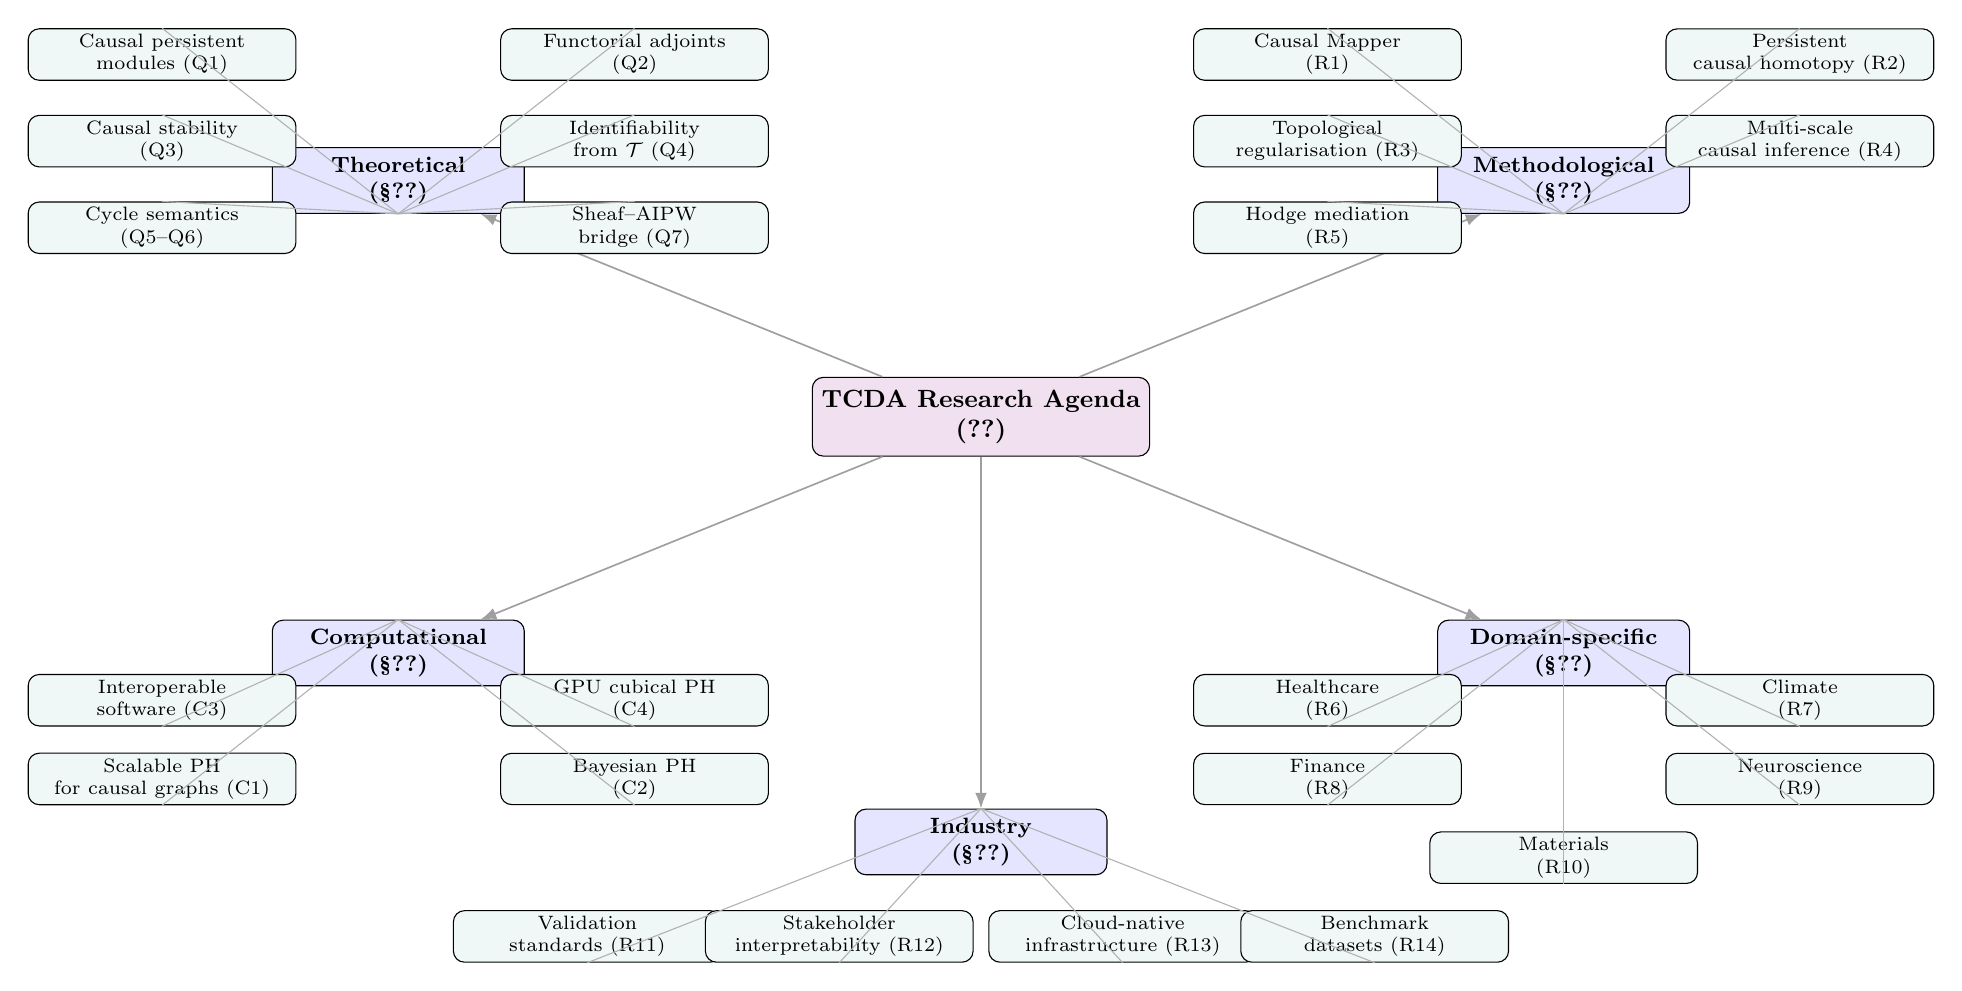
\begin{tikzpicture}[
    font=\footnotesize,
    every node/.style={align=center},
    centroid/.style={draw, rounded corners, fill=violet!12, minimum width=42mm,
                     minimum height=10mm, font=\small\bfseries},
    branch/.style={draw, rounded corners, fill=blue!10, minimum width=32mm,
                   minimum height=8mm, font=\footnotesize\bfseries},
    leaf/.style={draw, rounded corners, fill=teal!6, minimum width=34mm,
                 minimum height=6mm, inner sep=2pt, font=\scriptsize},
    edge from parent/.style={draw, semithick, -{Latex[length=2mm]}, gray!75}]

\node[centroid] (root) at (0, 0) {TCDA Research Agenda\\(\Cref{sec:research})};

\node[branch] (theory)   at ($(root) + (-7.4,  3.0)$) {Theoretical\\(\S\ref{sec:research_theory})};
\node[branch] (methods)  at ($(root) + ( 7.4,  3.0)$) {Methodological\\(\S\ref{sec:research_method})};
\node[branch] (compute)  at ($(root) + (-7.4, -3.0)$) {Computational\\(\S\ref{sec:research_compute})};
\node[branch] (domains)  at ($(root) + ( 7.4, -3.0)$) {Domain-specific\\(\S\ref{sec:research_domains})};
\node[branch] (industry) at ($(root) + ( 0.0, -5.4)$) {Industry\\(\S\ref{sec:research_industry})};

\draw[semithick, -{Latex[length=2mm]}, gray!75] (root) -- (theory);
\draw[semithick, -{Latex[length=2mm]}, gray!75] (root) -- (methods);
\draw[semithick, -{Latex[length=2mm]}, gray!75] (root) -- (compute);
\draw[semithick, -{Latex[length=2mm]}, gray!75] (root) -- (domains);
\draw[semithick, -{Latex[length=2mm]}, gray!75] (root) -- (industry);

% Theory leaves (upper-left)
\node[leaf] (t1) at ($(theory) + (-3.0, 1.6)$) {Causal persistent\\modules (Q1)};
\node[leaf] (t2) at ($(theory) + ( 3.0, 1.6)$) {Functorial adjoints\\(Q2)};
\node[leaf] (t3) at ($(theory) + (-3.0, 0.5)$) {Causal stability\\(Q3)};
\node[leaf] (t4) at ($(theory) + ( 3.0, 0.5)$) {Identifiability\\from $\Tc$ (Q4)};
\node[leaf] (t5) at ($(theory) + (-3.0,-0.6)$) {Cycle semantics\\(Q5--Q6)};
\node[leaf] (t6) at ($(theory) + ( 3.0,-0.6)$) {Sheaf--AIPW\\bridge (Q7)};
\foreach \x in {t1,t2,t3,t4,t5,t6} \draw[gray!60] (theory.south) -- (\x.north);

% Methods leaves (upper-right)
\node[leaf] (m1) at ($(methods) + (-3.0, 1.6)$) {Causal Mapper\\(R1)};
\node[leaf] (m2) at ($(methods) + ( 3.0, 1.6)$) {Persistent\\causal homotopy (R2)};
\node[leaf] (m3) at ($(methods) + (-3.0, 0.5)$) {Topological\\regularisation (R3)};
\node[leaf] (m4) at ($(methods) + ( 3.0, 0.5)$) {Multi-scale\\causal inference (R4)};
\node[leaf] (m5) at ($(methods) + (-3.0,-0.6)$) {Hodge mediation\\(R5)};
\foreach \x in {m1,m2,m3,m4,m5} \draw[gray!60] (methods.south) -- (\x.north);

% Compute leaves (lower-left)
\node[leaf] (c1) at ($(compute) + (-3.0,-1.6)$) {Scalable PH\\for causal graphs (C1)};
\node[leaf] (c2) at ($(compute) + ( 3.0,-1.6)$) {Bayesian PH\\(C2)};
\node[leaf] (c3) at ($(compute) + (-3.0,-0.6)$) {Interoperable\\software (C3)};
\node[leaf] (c4) at ($(compute) + ( 3.0,-0.6)$) {GPU cubical PH\\(C4)};
\foreach \x in {c1,c2,c3,c4} \draw[gray!60] (compute.north) -- (\x.south);

% Domain leaves (lower-right)
\node[leaf] (d1) at ($(domains) + (-3.0,-0.6)$) {Healthcare\\(R6)};
\node[leaf] (d2) at ($(domains) + ( 3.0,-0.6)$) {Climate\\(R7)};
\node[leaf] (d3) at ($(domains) + (-3.0,-1.6)$) {Finance\\(R8)};
\node[leaf] (d4) at ($(domains) + ( 3.0,-1.6)$) {Neuroscience\\(R9)};
\node[leaf] (d5) at ($(domains) + ( 0.0,-2.6)$) {Materials\\(R10)};
\foreach \x in {d1,d2,d3,d4,d5} \draw[gray!60] (domains.north) -- (\x.south);

% Industry leaves (bottom)
\node[leaf] (i1) at ($(industry) + (-5.0,-1.2)$) {Validation\\standards (R11)};
\node[leaf] (i2) at ($(industry) + (-1.8,-1.2)$) {Stakeholder\\interpretability (R12)};
\node[leaf] (i3) at ($(industry) + ( 1.8,-1.2)$) {Cloud-native\\infrastructure (R13)};
\node[leaf] (i4) at ($(industry) + ( 5.0,-1.2)$) {Benchmark\\datasets (R14)};
\foreach \x in {i1,i2,i3,i4} \draw[gray!60] (industry.north) -- (\x.south);

\end{tikzpicture}
\caption{Mind-map of the TCDA research agenda. The agenda has five
branches---theoretical (\Cref{sec:research_theory}), methodological
(\Cref{sec:research_method}), computational
(\Cref{sec:research_compute}), domain-specific
(\Cref{sec:research_domains}), and industry-facing
(\Cref{sec:research_industry})---comprising eleven formal Open
Questions (Q1--Q11), fourteen Research Avenues (R1--R14), and four
Computational Challenges (C1--C4). Each leaf is keyed to the formal
statement in the body of \Cref{sec:research}; together the leaves
populate every domain of the TCDA taxonomy (\Cref{fig:taxonomy}) with
at least one concrete, grant-scale open problem.}
\label{fig:research_mindmap}
\end{figure}


\subsection{Synthesis: a five-year and a ten-year horizon}
\label{sec:research_synth}

\Cref{fig:research_mindmap} aggregates the agenda. On a five-year
horizon, the most actionable items are the \emph{computational}
challenges of \Cref{sec:research_compute}---a working
\texttt{tcda-py} library, GPU cubical PH, scalable Vietoris--Rips---
together with the \emph{methodological} avenues of
\Cref{sec:research_method} that are within reach of existing
estimation theory: causal Mapper (\Cref{r:causal-mapper}),
topological regularisation (\Cref{r:topo-regularisation}), and Hodge
mediation (\Cref{r:hodge-mediation}). On a ten-year horizon, the
field's foundational identity will be settled by the \emph{theoretical}
questions of \Cref{sec:research_theory}: causal persistent modules
(\Cref{q:causal-modules}), functorial adjoints
(\Cref{q:adjoints}), a quantitative causal stability theorem
(\Cref{q:causal-stability}), the identifiability characterisation
(\Cref{q:tcda-identifiability}), and the sheaf-cohomological reading
of stability (\Cref{q:sheaf-aipw}). The domain-specific opportunities
of \Cref{sec:research_domains} and the industry items of
\Cref{sec:research_industry} are the empirical loci where the field
will earn its scientific standing.

Two observations close the section. First, every open question and
research avenue connects back to a gap identified in
\Cref{sec:lit_gaps} or to a remaining limitation noted in the case
studies of \Cref{sec:case_studies}: the agenda is not invented from
first principles but is the systematic completion of the existing
literature surveyed in \Cref{sec:literature}. Second, the agenda is
deliberately inclusive in scope and parsimonious in commitments: it
declares which problems matter without prescribing which solutions
will succeed, and so leaves room for a community of researchers from
both TDA and causal inference to enter the field on their own terms.
The next section---\Cref{sec:conclusion}---returns to the overall
vision and to the call for interdisciplinary collaboration that the
agenda enables.
}{}
\IfFileExists{sections/conclusion.tex}{\section{Conclusion}\label{sec:conclusion}

We have proposed \emph{Topological Causal Data Analysis} as a
coherent research domain at the intersection of two mature
mathematical traditions. The case for the proposal rests on four
elements that the body of the paper has developed in turn: a formal
framework (\Cref{sec:framework}) anchored in the tuple
$(\Mc, G, \Tc, \Cc)$ of \Cref{def:tcda} and the foundational
propositions \Cref{prop:stability-transfer,prop:identifiability}; a
structured literature review (\Cref{sec:literature}) showing that the
methodological building blocks of TCDA are already in place but
fragmented across five non-interacting threads
(\Cref{sec:lit_gaps}); a suite of five case studies
(\Cref{sec:case_studies}) demonstrating that the framework is
non-vacuous and that each cell of its taxonomy admits an explicit
instantiation; and a research agenda (\Cref{sec:research}) comprising
eleven formal Open Questions, fourteen Research Avenues, and four
Computational Challenges calibrated against the gaps and case-study
limitations identified earlier.

\paragraph{The four cornerstones of the field.}
The argument of the paper is that the four seed works
$\{$\citet{ibeling2021topological}, \citet{kim2026topological},
\citet{lecci2014statistical},
\citet{elyaagoubi2023statistical}$\}$, taken together, span the
mathematical, statistical, and methodological corners of TCDA. The
first supplies the topology of causal-model spaces and the
no-free-lunch theorem that frames the field's negative results
\citep{ibeling2021topological}; the second supplies the
doubly-robust, stability-guaranteed estimator that converts a
topological summary into a calibrated causal quantity
\citep{kim2026topological}; the third supplies the statistical
inference scaffolding---confidence sets, bootstrap, rates of
convergence---without which the calibration of \emph{any} TCDA
estimator would be void \citep{lecci2014statistical}; and the fourth
supplies the simulation-based benchmark on which discovery procedures
in time-series and dependence-network settings can be evaluated
\citep{elyaagoubi2023statistical}. No single seed work is the field
on its own, and a serious TCDA programme must draw on all four
threads in parallel.

\paragraph{What we have not done.}
We have not claimed that the framework is final, that every
proposition is fully proved, that every open question is solvable on
its current statement, or that the taxonomy is mutually exclusive.
Several arguments in \Cref{sec:framework,sec:case_studies} are
proof sketches that demand fuller treatment, several research
avenues in \Cref{sec:research} are likely to fragment or merge as
the field matures, and the case studies of \Cref{sec:case_studies}
sit at varying levels of methodological readiness---some are
recapitulations of published work, others are concrete proposals
awaiting implementation. The four contributions enumerated in
\Cref{sec:intro_contributions} should therefore be understood as a
proposal in the technical sense---a unified vocabulary, a
taxonomy, a literature map, and an agenda---rather than as a
declaration of completion.

\paragraph{A call for interdisciplinary collaboration.}
The community most likely to settle the open questions of
\Cref{sec:research} does not yet exist. Its constituents---algebraic
topologists, statisticians, machine-learning researchers, causal-
inference theorists, computational scientists, and domain experts in
biomedicine, climate, finance, neuroscience, and materials---are
distributed across departments that historically have not shared
seminars or journals. The contribution that TCDA can make beyond its
internal technical agenda is to provide a vocabulary in which
collaborations across these silos can be staged: a topologist can
read \Cref{prop:stability-transfer} as a stability statement and
contribute new admissible functors $\Tc$; a causal-inference theorist
can read \Cref{prop:identifiability} as an identifiability question
and contribute new classes $\mathcal{G}$; a domain scientist can read
the case studies of \Cref{sec:case_studies} as templates and
contribute new applications; a computational scientist can read
\Cref{sec:research_compute} as a list of engineering targets. The
challenges that result---the GPU cubical PH of
\Cref{c:gpu-cubical}, the interoperable software of
\Cref{c:software}, the benchmark suite of \Cref{r:benchmarks}, the
validation standards of \Cref{r:validation-standards}---are
themselves invitations to a kind of work that no single sub-community
can complete in isolation. We hope this paper makes such invitations
easier to extend and easier to accept.

\paragraph{Closing.}
The slogan we offer is simple: \emph{the shape of data has a causal
story to tell}. Topology, on its own, recovers the shape; causal
inference, on its own, recovers the story; and only together can they
deliver, for the increasingly complex and increasingly non-Euclidean
data of contemporary science, the calibrated and intervention-aware
accounts that practical deployment demands. The four contributions of
this paper---a framework, a literature, a case-study suite, and an
agenda---are offered as the starting point of that joint enterprise,
not its conclusion. The body of work that converts the proposal into
a mature field remains to be done, and it is to that body of work
that we hope this paper now invites the reader.
}{}

\bibliographystyle{plainnat}
\bibliography{bibliography}

\end{document}
